\documentclass{article}

\usepackage{arxiv}
\usepackage[utf8]{inputenc}
\usepackage[T1]{fontenc}

% Zotero-exported bib entries occasionally contain unmapped Unicode codepoints.
% Map them so pdflatex can typeset them without failing.
\DeclareUnicodeCharacter{03A6}{\ensuremath{\Phi}}
\DeclareUnicodeCharacter{0131}{\i}
\DeclareUnicodeCharacter{015F}{\c{s}}
\DeclareUnicodeCharacter{0302}{\^{}}
\usepackage{hyperref}
\usepackage{url}
\usepackage{booktabs}
\usepackage{amsfonts}
\usepackage{amsmath}
\usepackage{amssymb}
\usepackage{nicefrac}
\usepackage{microtype}
\usepackage{graphicx}
\usepackage[numbers]{natbib}
\usepackage{doi}
\usepackage{pgfplots}
\usepackage{tikz}
\usepackage{siunitx}
\usepackage{subcaption}
\usepackage{algorithm}
\usepackage{algpseudocode}
\usepackage{todonotes}
\usepackage{fontawesome5}
\usepackage{placeins}
\usepackage{amsthm}

\newtheorem{proposition}{Proposition}
\newtheorem{lemma}[proposition]{Lemma}
\newtheorem{corollary}[proposition]{Corollary}
\newtheorem{definition}[proposition]{Definition}
\theoremstyle{remark}
\newtheorem{remark}[proposition]{Remark}

\usetikzlibrary{arrows.meta, positioning, shapes.geometric, calc, decorations.markings, patterns, fit, backgrounds, angles, quotes}
\usepgfplotslibrary{groupplots}
\pgfplotsset{compat=1.18}

\newcommand{\vect}[1]{\mathbf{#1}}
\newcommand{\mat}[1]{\mathbf{#1}}
\newcommand{\R}{\mathbb{R}}
\DeclareMathOperator*{\argmin}{argmin}

\newcommand\figref{Figure~\ref}
\renewcommand\eqref{Equation~\ref}
\newcommand\tabref{Table~\ref}
\newcommand*{\secref}[1]{\hyperref[{#1}]{\S\ref*{#1}}}

\title{Look Before You Slew: Information-Gated Dynamic Tasking for Agile Earth Observation}

\author{\normalfont
\href{https://orcid.org/0000-0002-7227-4946}{
\includegraphics[scale=0.06]{orcid.pdf}\hspace{1mm}\textbf{Shreeyam Kacker}}\textsuperscript{1}
\quad \textbf{Steve Chien}\textsuperscript{2}
\quad \textbf{Işıl Demir}\textsuperscript{3}
\quad \textbf{Kiruthika Devaraj}\textsuperscript{3}
\quad \textbf{Kerri Cahoy}\textsuperscript{1}\\[0.35em]
\textsuperscript{1}Department of Aeronautics and Astronautics, MIT\\
\textsuperscript{2}Jet Propulsion Laboratory, California Institute of Technology\\
\textsuperscript{3}Planet Labs\\
\texttt{shreeyam@mit.edu} \quad \texttt{kcahoy@mit.edu}
}

\renewcommand{\headeright}{}
\renewcommand{\undertitle}{}
\renewcommand{\shorttitle}{Look Before You Slew}

\hypersetup{
pdftitle={Look Before You Slew: Information-Gated Dynamic Tasking for Agile Earth Observation},
pdfsubject={astro-ph, cs.AI},
pdfauthor={Shreeyam Kacker, Steve Chien, Işıl Demir, Kiruthika Devaraj, Kerri Cahoy},
pdfkeywords={dynamic tasking, Earth observation, spacecraft scheduling, value of information, active perception, onboard autonomy},
}

\begin{document}
\maketitle

\begin{abstract}
\input{sections/abstract}
\end{abstract}

\noindent\textbf{Keywords:} dynamic tasking, Earth observation, spacecraft scheduling, onboard autonomy, agile satellites

\noindent\faGithub\hspace{0.5em}\url{https://github.com/Shreeyam/phd_code}

\section{Introduction}
\label{sec:introduction}

Modern Earth-observing (EO) satellites, while significantly more capable than those of the past, are still frequently operated with little autonomy: schedules are optimized on the ground, uplinked before execution, and then followed with limited ability to react to uncertain events in orbit.
This mode of operation is effective when target values are known or can be accurately forecasted, but is inefficient when planning under uncertainty.
Wildfires, volcanic eruptions, floods, storms, and other transient events can change where observations are valuable after a schedule is uplinked. The most common detractor of imaging is cloud cover---clouds occlude approximately 66\% of Earth's surface at any time~\citep{king_spatial_2013}, and if the objective is not to observe clouds, many scheduled imaging activities produce little value even when the pre-planned schedule is followed perfectly.

Dynamic targeting addresses this limitation by using onboard observations to re-optimize the schedule onboard.
We consider the case of a spacecraft with a secondary, body-fixed, wide-field instrument that observes upcoming targets, an onboard classifier estimates updated utility values, and the scheduler re-optimizes the schedule based on new information.
\figref{fig:conops} contrasts this onboard dynamic-tasking loop with conventional fixed-schedule execution.

\begin{figure}[t]
    \centering
    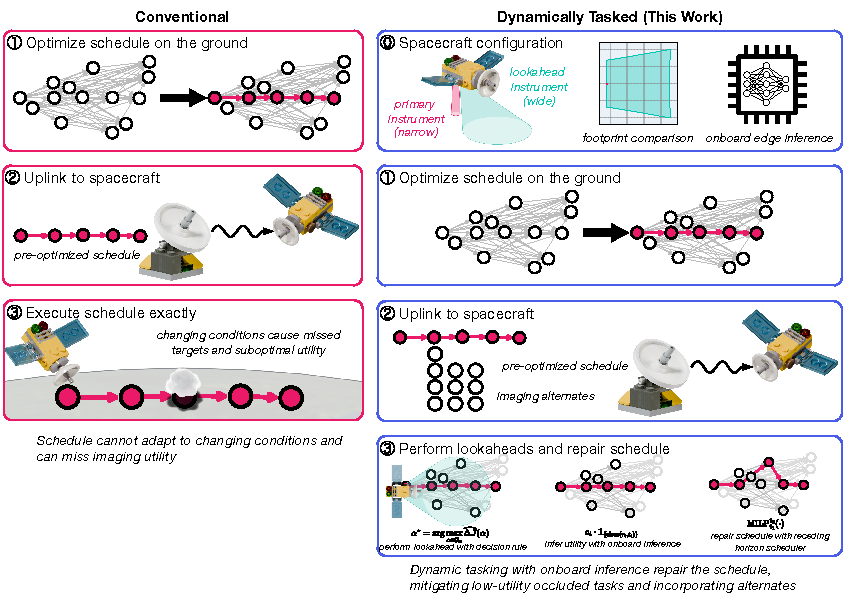
\includegraphics[width=\linewidth]{figures/dt_overview_new.pdf}
    \caption{Dynamic tasking concept of operations. \textbf{(left)} Conventional operations optimize and uplink a fixed schedule; when cloud state or task utility changes, the spacecraft may execute low-value collects. \textbf{(right)} In this work, a body-fixed wide-field lookahead instrument observes upcoming accesses, onboard inference updates candidate access utilities, and a receding-horizon scheduler repairs the local schedule before the primary imager commits.}
    \label{fig:conops}
\end{figure}

However, acquiring new information can come with its own costs---performing a lookahead can reveal viable alternative activities, but can consume slew time and may displace scheduled imaging, as well as inference time.
The utility of a lookahead action is therefore how much the schedule utility improves by, taking into account all gains and resource costs.

This makes body-fixed lookahead a value-of-information problem: the spacecraft is not simply choosing the next image, but choosing whether an attitude maneuver that gathers information will improve the downstream schedule enough to justify its cost.
Previous work often searches directly over lookahead actions or assumes a fixed observation strategy~\citep{kangaslahti_dynamic_2024, candela_dynamic_2022}, while in this work we frame dynamic tasking as decision analysis under flight-system constraints. We consider the bounding cases of a theoretical omniscient scheduler with perfect advance information, and a conventional scheduler executing a pre-planned schedule without deviation. The gap between them is therefore the expected value of perfect information (EVPI), and the gap closed by any dynamic tasking policy is its expected value of sample information (EVSI)~\citep{howard_information_1966, raiffa_applied_1968}.

Every contribution in this paper can be read through that lens: the systems analysis defines which information-gathering actions are physically available, the break-even utility rule decides whether those actions can repay their local schedule burden, and the timing and pointing rules maximize that margin over a schedule gap.

We make the following contributions:
\begin{enumerate}
    \item A \textbf{systems analysis} of body-fixed lookahead sensing for agile EO satellites, relating ConOps, field of view, geometry, and agility to the feasible information-gathering action space (\secref{sec:systems_analysis}).
    \item A \textbf{two-anchor renewal value model} for lookahead actions, plus a monotone break-even approximation that computes the maximum dead time each candidate pointing angle can tolerate and accepts the best angle only when that threshold exceeds the physical slew cost (\secref{sec:heuristic}).
    \item A \textbf{receding-horizon control loop} that combines camera projection, break-even pointing search, optimal maneuver timing, and local schedule repair into an onboard dynamic-tasking policy (\secref{sec:lookahead_policy}--\secref{sec:schedule_repair}).
\end{enumerate}

\paragraph{Paper organization.}
We review prior work on spacecraft scheduling, dynamic tasking, active perception, and sequential information acquisition (\secref{sec:background}), then analyze the spacecraft ConOps, request-to-access abstraction, field-of-view geometry, and agility constraints that reduce body-fixed lookahead tasking to a local onboard decision (\secref{sec:systems_analysis}). We then develop the break-even spacing rule, optimal timing and pitch search, and schedule repair loop that implement that decision (\secref{sec:method}). We close (\secref{sec:conclusion}) with the scope of the unit-utility, perfect-classification, and non-uniform request-utility assumptions.

\section{Background}
\label{sec:background}

\paragraph{EO scheduling.}
We consider the problem of a single agile EO satellite that selects a feasible subset of requested images to maximize collected utility.
Following conventions in previous EO scheduling work~\citep{augenstein_optimal_2014, eddy_task_2021}, each request consisting of a latitude/longitude point is combined with the satellite orbital parameters to produce a list of accesses: a tuple of the request, time, and off-nadir roll angle \cite{kacker_spacecraft_2025}. A mixed integer linear program (MILP) is then used to schedule these accesses subject to agility and repetition constraints \secref{sec:scheduling}.

Prior scheduling work for agile EO spacecraft varies on runtime, optimality, and expressivity.
Greedy dispatch rules are simple enough for onboard use~\citep{bianchessi_heuristic_2007, bianchessi_planning_2008, wolfe_three_2000}, while MILP formulations provide optimal schedules for known utilities~\citep{bensana_earth_1999, augenstein_optimal_2016, nag_autonomous_2019}.
Graph-based longest-path and maximum-independent-set formulations exploit the sparse structure of access conflicts for near-optimal solutions at lower cost~\citep{augenstein_optimal_2014, eddy_maximum_2021, eddy_task_2021}.
Markov decision process (MDP), reinforcement-learning (RL), and Monte Carlo tree search approaches have been explored and need not stick to the access-based formulation~\citep{eddy_markov_2020, herrmann_reinforcement_2023, wang_deep_2023, hadj-salah_schedule_2019, herrmann_monte_2022}. 

% but the central obstacle for dynamic tasking is not only schedule optimization: it is deciding which uncertain future accesses are worth observing before the primary instrument commits.

\paragraph{Dynamic targeting and tasking.}
We use dynamic \emph{targeting} for systems that acquire new information and synthesize new imaging targets within a single overflight, and dynamic \emph{tasking} for the case of re-optimizing with an initial schedule and a fixed list of requests.
EO-1's Autonomous Sciencecraft Experiment (ASE) pioneered onboard replanning and onboard ML-based classification, though its compute budget restricted autonomy primarily to follow-up observations rather than within-overflight replanning~\citep{chien_using_2005, chien_lessons_2005, wagstaff_cloud_2017} .
More recent systems are able to re-plan within a single overflight: GOSAT-2 re-points its primary instrument away from clouds using a fold mirror~\citep{imasu_greenhouse_2023}, and CogniSAT-6 demonstrated autonomous tasking on a 6U CubeSat using a CNN pipeline on a Myriad~X VPU~\citep{rijlaarsdam_autonomous_2024}.

Algorithmic work has addressed onboard replanning with anytime planners, timeline fragments, pointing heuristics, constellation-aware MILPs, and MDPs~\citep{damiani_continuous_2005, lenzen_onboard_2014, chien_heuristic_nodate, chien_onboard_2015, nag_autonomous_2019, candela_dynamic_2022}.
Kangaslahti et al.~\citep{kangaslahti_dynamic_2024} provide the closest robotics-side satellite comparator, modeling dynamic targeting with a lookahead sensor, slewing constraints, changing observation utility, and greedy/depth-first search over observation choices.
These methods establish onboard adaptation, but generally either search directly over lookahead actions or assume a fixed observation strategy rather than deriving the lookahead decision space from spacecraft geometry and agility constraints and then attaching a lightweight value-of-information gate.
Complementary threads in our own prior work explored learned lookahead heuristics~\citep{kacker_reinforcement-learned_2024} and dynamic tasking driven by real-time GEO meteorological data~\citep{kacker_leveraging_2025}.
% The remaining gap is a lightweight value model for body-fixed lookahead that can be evaluated onboard and tied to formal timing guarantees.

\paragraph{Onboard compute and agility.}
\label{sec:compute}
\label{sec:agility_background}
Vision-based dynamic tasking requires enough onboard compute to classify lookahead imagery before the target passes.
This was prohibitive for EO-1's ${\sim}4$~MIPS shared flight processor~\citep{chien_using_2005, chien_lessons_2005}, but recent COTS VPU/GPU-class processors support in-orbit ML, onboard cloud detection, compression, and autonomous tasking demonstrations~\citep{kacker_machine_2022, giuffrida_-sat-1_2022, marin_phi-sat-2_2021, rijlaarsdam_autonomous_2024, rijlaarsdam_next_2024, noauthor_planet_2024}.
For this paper, classification is no longer the tight loop; schedule repair time and spacecraft agility are.

Agility determines whether information from a lookahead can still be acted on before the primary imaging opportunity passes~\citep{eddy_task_2021, lemaitre_selecting_2002}.
Most representative agile platforms complete this maneuver in 25--40~s with a $\pm$\ang{45} off-nadir field of regard.
Representative public slew specifications are summarized in Appendix~\ref{sec:appendix_system_data}.
A practical lookahead instrument must span the field of regard horizontally and provide tens of seconds of vertical lead time; \secref{sec:lookahead_design} derives these geometry constraints.

\paragraph{Sequential information acquisition.}
Dynamic tasking can be viewed as sequential information acquisition: the spacecraft spends time and resources to reveal uncertain task values before committing the primary instrument.
In robotics, the analogous active-perception and informative-path-planning problems choose sensing actions under travel, time, or energy constraints, often trading exploration against exploitation in a partially observed environment~\citep{singh_nonmyopic_2009, tan_informative_2024}.
Those formulations usually value observations through uncertainty reduction, coverage, or submodular information objectives.
Classical inspection and probing models study related value-of-information trade-offs~\citep{weitzman_optimal_1978, gupta_algorithms_2015}, but they typically treat inspected items as separable.
EO tasking differs from both threads because the value of a revealed clear target depends on whether it can be inserted into a feasible schedule. This coupling between information value, spacecraft agility, and schedule repair is the setting considered in this paper.

\section{Systems Analysis}
\label{sec:systems_analysis}

The algorithm is derived from the flight-system constraints.
Rather than solve an adaptive stochastic scheduling problem with continuous lookahead times, continuous pointing angles, unknown cloud states, and a combinatorial imaging schedule, we first use spacecraft geometry and agility limits to collapse dynamic tasking into local decisions made in schedule gaps.
For each gap, the spacecraft asks whether one lookahead maneuver is physically meaningful and, if so, what pitch angles are feasible.
The lookahead decision method in the next section then estimates whether any feasible maneuver has positive schedule-level value.

\subsection{Dynamic Tasking Formulation}
\label{sec:dt_formulation}

Conventional scheduling treats access utilities $u_i$ as known. In practice they are modulated by cloud state:
\begin{equation}
u_i = c_i \cdot \mathbf{1}_{\{\text{clear}(r_i, t_i)\}},
\end{equation}
where $c_i$ is intrinsic value and $\mathbf{1}_{\{\cdot\}}$ indicates cloud-free conditions.
We focus on the \emph{unit-utility} case ($c_i = 1$), isolating when to look from task-value heterogeneity; the heavy-tailed utility regime is treated in~\cite{kacker_spacecraft_2025}.
Cloud state is unknown when the ground schedule is produced, but can be revealed by a \emph{lookahead observation} that points a secondary wide-field instrument toward upcoming targets and triggers schedule repair with updated utilities.

A lookahead therefore has two coupled effects: \emph{advantage} from revealing clear accesses that may be inserted into the repaired schedule, and \emph{opportunity cost} from consuming slew time that could otherwise be used for imaging.
The systems problem is to decide which lookahead actions are physically meaningful; the algorithmic problem is to estimate whether their expected advantage exceeds their cost using only onboard information.

This paper analyzes the body-fixed onboard-lookahead case because it is the most tightly coupled to spacecraft agility: the same bus that images targets must also slew to acquire information about them.
Other dynamic-tasking architectures, including leader-follower constellations, sensor webs, and real-time meteorological-data feeds, shift this trade to communication latency, sensor cadence, and data-fusion assumptions~\citep{chien_autonomous_2005, chien_automated_2020, chien_using_2019, kacker_leveraging_2025, mahonchak_goes-r_nodate}.
The body-fixed case therefore provides a constrained reference problem in which field of view, horizon lead time, and slew time directly determine the feasible onboard decision space.

\subsection{Baseline Scheduling Model}
\label{sec:scheduling}

An Earth-observing satellite receives imaging requests $\mathcal{R}$ and, given an orbit, converts each request into a set of \emph{accesses} $\mathcal{A}$.
Operational requests may be point, strip, or area collects; for this analysis they are represented as point access opportunities, following the standard EO scheduling pipeline that tessellates or decomposes requests before access generation~\citep{eddy_task_2021, xu_multi-satellite_2020}.
Each access $a_i = (r_i, t_i, \theta_i)$ records the request, overpass time, and off-nadir roll angle, following~\cite{eddy_task_2021}.
The scheduling problem is to select a subset $\boldsymbol{\sigma} \subseteq \mathcal{A}$ maximizing total utility subject to agility constraints:
\begin{equation}
\max_{\boldsymbol{\sigma}} \sum_{a_i \in \boldsymbol{\sigma}} u_i, \quad
\text{s.t.} \quad t_j - t_i \geq t_{\mathrm{slew}}(\theta_j - \theta_i) \;\;\forall\; a_i, a_j \in \boldsymbol{\sigma},\; t_j > t_i,
\label{eq:scheduling}
\end{equation}
where the slew time follows a bang-bang agility model $t_{\mathrm{slew}}(\Delta\theta) = t_s + \beta\sqrt{|\Delta\theta|}$, with settling time $t_s$ and rate parameter $\beta$.
We solve~\eqref{eq:scheduling} via mixed-integer linear programming (MILP), with an additional repetition constraint preventing multiple accesses of the same request.

\subsection{Lookahead Geometry and Agility Constraints}
\label{sec:lookahead_design}

We consider a body-fixed secondary instrument pointed ahead of nadir toward the horizon.
The systems design determines the algorithmic action space: a lookahead action is feasible only if its field of view covers useful future accesses and the spacecraft can complete the maneuver before the next scheduled image.
Two assumptions fix the geometry: the spacecraft's neutral position after imaging is nadir-pointed, and the lookahead field of view has its bottom edge at nadir (so boresight pitch equals half the vertical FoV).
This is intentionally the constrained case: electronically steerable lookahead sensors, fold mirrors, and radar-based sensing can partially decouple observation from bus agility~\citep{imasu_greenhouse_2023, bosch-lluis_smart_2022}, but a body-fixed payload makes the agility and field-of-view requirements explicit.

\paragraph{Spherical geometry.}
Let $a = R_E + h$ be the orbital radius and $n = \sqrt{\mu/a^3}$ the mean motion.
A point at the horizon reaches nadir after
\begin{equation}
t_{\mathrm{horizon}} = \frac{1}{n} \arccos\!\left(\frac{R_E}{a}\right),
\label{eq:horizon}
\end{equation}
giving $t_{\mathrm{horizon}} \approx \SI{305}{\second}$ at $h = \SI{400}{\kilo\metre}$ and bounding the maximum observation lead time.
In \figref{fig:lookahead_geometry}, a ray from spacecraft $S$ pitched ahead by angle $\alpha$ intersects Earth at $P$ and subtends the Earth-centered angle $\angle NOP$:
\begin{equation}
\psi(\alpha) = \arccos\!\left(\frac{a\sin^2\alpha + \cos\alpha\,\sqrt{R_E^2 - a^2 \sin^2\alpha}}{R_E}\right)
\label{eq:dtrack}
\end{equation}
from nadir and reaches nadir after $t_{\mathrm{point}}(\alpha) = \psi(\alpha)/n$.
The same ray intersection also has a local coordinate in the plane through $N$ tangent to the local horizontal:
\begin{equation}
\rho(\alpha) =
\sin\alpha \left[a\cos\alpha -
\sqrt{R_E^2 - a^2 \sin^2\alpha}\right].
\label{eq:ground_offset}
\end{equation}
In the diagram, $\psi(\alpha)$ is the central angle $\angle NOP$.
The companion flat-plane quantity $\rho(\alpha)$ is the local-horizontal projection of $NP$: the signed distance, in the plane tangent to Earth at $N$, from $N$ to the projection of $P$ along the local vertical direction $ON$.
It is therefore not the curved ground distance along the surface, but the coordinate used to place ray hits in the local detector geometry below.
The same spherical setup is used below for both lookahead timing and field-of-view sizing.

\begin{figure}[htb]
    \centering
    \begin{subfigure}[b]{0.36\textwidth}
        \centering
        \raisebox{1.2em}{%
        \resizebox{\linewidth}{!}{%
        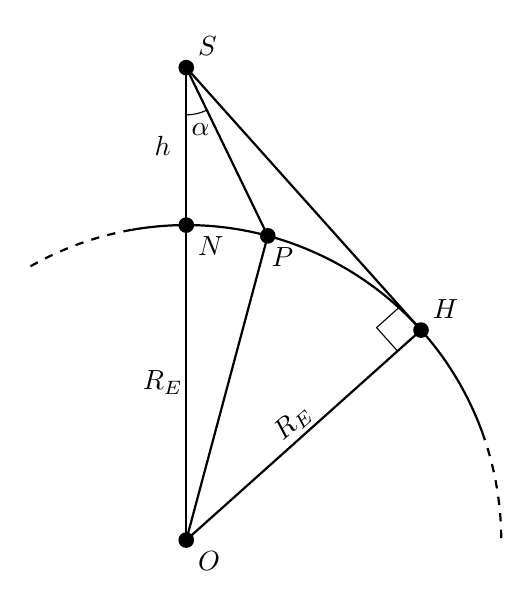
\begin{tikzpicture}[
            dot/.style = {circle, fill=black, inner sep=2pt},
            lbl/.style = {label distance=-0.7mm},
            >=latex]
            \def\r{4}
            \def\dphi{20}
            \coordinate (O) at (0,0);
            \coordinate (S) at (0,1.5*\r);
            \coordinate (P) at ({\r*cos 75},{\r*sin 75});
            \coordinate (H) at ({\r*sqrt(5)/3},{2*\r/3});
            \coordinate (N) at (0,\r);
            \draw[thick,dashed] ({\r*cos 100},{\r*sin 100})
                arc[start angle=100,end angle=100+\dphi,radius=\r];
            \draw[thick] ({\r*cos 100},{\r*sin 100})
                arc[start angle=100,end angle=20,radius=\r];
            \draw[thick,dashed] ({\r*cos 20},{\r*sin 20})
                arc[start angle=20,end angle=20-\dphi,radius=\r];
            \draw[thick] (S) -- (N) node[midway,xshift=-3mm] {$h$};
            \draw[thick] (N) -- (O) node[midway,xshift=-3mm] {$R_E$};
            \draw[thick] (O) -- (H) node[midway,sloped,above=-0.7mm] {$R_E$};
            \draw[thick] (H) -- (S);
            \draw[thick] (O) -- (P) -- (S);
            \pic [draw, angle radius=4mm] {right angle = O--H--S};
            \pic [draw, angle radius=6mm, "$\alpha$", angle eccentricity=1.35] {angle = N--S--P};
            \node[dot,label={[lbl]below right:$O$}] at (O) {};
            \node[dot,label={[lbl]above right:$S$}] at (S) {};
            \node[dot,label={[lbl, xshift=-1mm]below right:$P$}] at (P) {};
            \node[dot,label={[lbl]above right:$H$}] at (H) {};
            \node[dot,label={[lbl]below right:$N$}] at (N) {};
        \end{tikzpicture}%
        }}
        \caption{Spherical geometry.}
        \label{fig:lookahead_geometry}
    \end{subfigure}
    \hfill
    \begin{subfigure}[b]{0.6\textwidth}
        \centering
        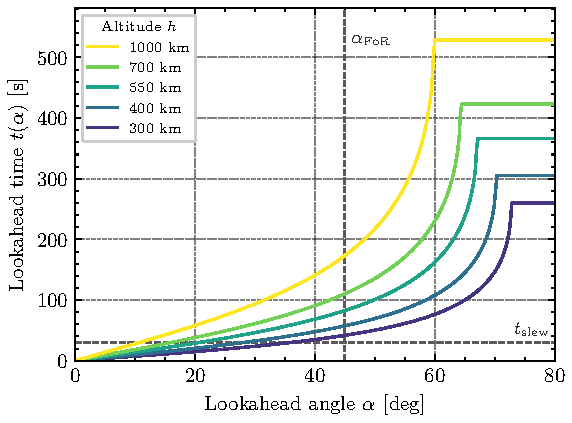
\includegraphics[width=\textwidth]{figures/lookahead_time_constraints.pdf}
        \caption{Lookahead time over altitude.}
        \label{fig:lookahead_time_altitudes}
    \end{subfigure}
    \caption{Lookahead geometry and timing. \textbf{(a)} Spacecraft at $S$, nadir projection $N$, horizon tangent $H$, and target $P$ at pitch angle $\alpha$. The central angle $\angle NOP$ is $\psi(\alpha)$, while the local-horizontal projection of $NP$ is $\rho(\alpha)$. \textbf{(b)} Lookahead time $t(\alpha)$ for representative LEO altitudes. A lookahead is actionable where $t(\alpha) \geq t_{\mathrm{slew}}$ and $\alpha \leq \alpha_{\mathrm{FoR}}$.}
    \label{fig:lookahead_time_constraints}
\end{figure}

\paragraph{Vertical FoV.}
Three timing constraints act on the vertical FoV:
\begin{itemize}
    \item \textbf{Slew time:} the instrument must see ahead far enough that every task within the off-nadir field of regard is still reachable after a full cross-track slew.
    \item \textbf{Pitching field of regard:} in the worst case---pitched fully backward within the field of regard---the instrument must still observe beyond nadir.
    \item \textbf{Settling time:} even when a task is visible, the maneuver plus settling may leave no feasible action, defining regions where a lookahead is \emph{never} net-positive.
\end{itemize}
\figref{fig:lookahead_time_constraints} plots $t(\alpha)$ across LEO altitudes. A lookahead is actionable only where $t(\alpha) \geq t_{\mathrm{slew}}$ and $\alpha \leq \alpha_{\mathrm{FoR}}$.

\paragraph{Horizontal FoV.}
Horizontal constraints depend on the primary imager field of regard $\theta_{\mathrm{FoR}}$ and take two forms:
\begin{itemize}
    \item \textbf{Nadir FoR:} both edges of the field of regard must lie within the sensor FoV when the spacecraft is at nadir.
    \item \textbf{Rolled FoR:} the lookahead footprint must reach the field-of-regard edges when the spacecraft is rolled to the maximum off-nadir angle to acquire an image.
\end{itemize}
Let $\Theta_h$ denote the full horizontal FoV and let $\beta=\Theta_v/2$.
The horizontal calculation reuses the same plane tangent at $N$ in \figref{fig:lookahead_geometry}, but now with one local-horizontal coordinate $x$ forward along track and one coordinate $y$ cross track.
The coordinate $x$ is the same type of local-horizontal projection as $\rho(\alpha)$ in the spherical-geometry paragraph.
A primary-imager FoR edge has cross-track projection $\rho_F=\rho(\theta_{\mathrm{FoR}})$, so points on the two FoR edges have local-horizontal coordinates $(x,\pm\rho_F)$ before detector projection.
\figref{fig:tangent_plane_frame} summarizes this local frame.

\begin{figure}[htbp]
    \centering
    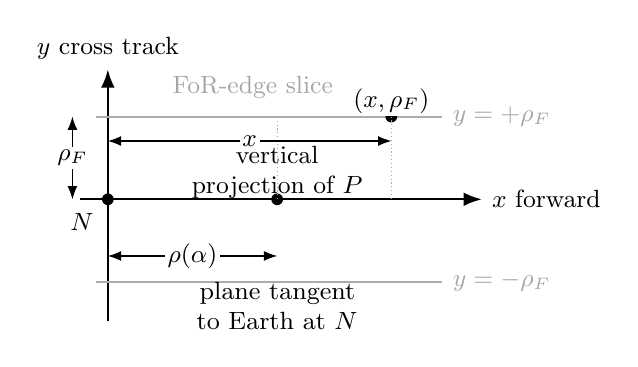
\begin{tikzpicture}[
        >=Latex,
        x=1cm,
        y=1cm,
        point/.style={circle, fill=black, inner sep=1.5pt},
        edge/.style={thick, gray!65},
        guide/.style={densely dotted, gray!70},
        lbl/.style={font=\small}
    ]
        \coordinate (N) at (0,0);
        \coordinate (Pproj) at (2.15,0);
        \coordinate (Q) at (3.6,1.05);

        \draw[->, thick] (-0.35,0) -- (4.75,0) node[right,lbl] {$x$ forward};
        \draw[->, thick] (0,-1.55) -- (0,1.65) node[above,lbl] {$y$ cross track};

        \draw[edge] (-0.15,1.05) -- (4.25,1.05) node[right,lbl, gray!70] {$y=+\rho_F$};
        \draw[edge] (-0.15,-1.05) -- (4.25,-1.05) node[right,lbl, gray!70] {$y=-\rho_F$};
        \node[lbl, gray!70, anchor=west] at (0.7,1.42) {FoR-edge slice};

        \node[point,label={[lbl]below left:$N$}] at (N) {};
        \node[point] at (Pproj) {};
        \node[lbl, align=center] at (2.15,0.34) {vertical\\projection of $P$};
        \node[point] at (Q) {};
        \node[lbl, anchor=south, fill=white, inner sep=1pt] at (Q) {$(x,\rho_F)$};

        \draw[guide] (Pproj) -- ++(0,1.05);
        \draw[guide] (Q) -- ++(0,-1.05);
        \draw[<->] (0,-0.72) -- node[fill=white, inner sep=1pt, lbl] {$\rho(\alpha)$} (2.15,-0.72);
        \draw[<->] (-0.45,0) -- node[fill=white, inner sep=1pt, lbl] {$\rho_F$} (-0.45,1.05);
        \draw[<->] (0,0.74) -- node[fill=white, inner sep=1pt, lbl] {$x$} (3.6,0.74);

        \node[lbl, align=center, text width=3.6cm] at (2.15,-1.35)
            {plane tangent to Earth at $N$};
    \end{tikzpicture}
    \caption{Local tangent-plane frame used for horizontal-FoV sizing. The spherical diagram defines $N$ and $P$; here $P$ is projected onto the plane tangent at $N$ along the local vertical direction $ON$. The primary-imager FoR edges become the two lines $y=\pm\rho_F$, and fixing one edge gives the Earth slice used to define $R_F$ and $z(x)$.}
    \label{fig:tangent_plane_frame}
\end{figure}

The corresponding fixed-FoR-edge Earth slice has radius and nadir-axis depth
\begin{equation}
R_F=\sqrt{R_E^2-\rho_F^2},\qquad
z(x)=a-\sqrt{R_F^2-x^2}.
\label{eq:for_edge_slice}
\end{equation}
The subscript $F$ denotes this fixed FoR-edge slice.
Here $z(x)$ is the component of the vector from $S$ to the surface point along the spacecraft-nadir direction $SN$.
The analogue of horizon point $H$ on one of these fixed-FoR-edge slices is the limb point on that FoR edge: the point where the ray from $S$ is tangent to Earth.
Its forward coordinate is
\begin{equation}
x_{\mathrm{limb}}=\sqrt{R_E^2\left(1-\left[\frac{R_E}{a}\right]^2\right)-\rho_F^2}.
\label{eq:for_horizon_cap}
\end{equation}
Thus $x_{\mathrm{limb}}$ is not a field-of-view angle: detector contacts beyond it are physically beyond Earth and are replaced by the limb point on the same FoR edge.
Once $\Theta_v$ is chosen, the forward edge of the lookahead lies at off-nadir angle $\Theta_v$ because the lower edge is fixed at nadir.
Both horizontal constraints are obtained by projecting the two FoR edges into the same rectilinear detector plane; Appendix~\ref{sec:appendix_fov_projection} gives the shared map.
The useful closed forms below are the nadir and rolled specializations of that map.

For the nadir attitude, $\varphi=0$ and the two FoR edges are symmetric.
The limiting forward coordinate is the first contact between the upper detector edge and the FoR edge, unless that contact lies past the limb:
\begin{equation}
\begin{aligned}
\Theta_v^{\mathrm{limb}}
&=\arcsin\!\left(\frac{R_F}{a}\right),\\
x_{\mathrm{edge}}
&=\sin\Theta_v
\left[
a\cos\Theta_v
-\sqrt{R_F^2-a^2\sin^2\Theta_v}
\right],\\
x_{\mathrm{nadir}}
&=
\begin{cases}
x_{\mathrm{edge}}, & \Theta_v\leq\Theta_v^{\mathrm{limb}},\\
x_{\mathrm{limb}}, & \Theta_v>\Theta_v^{\mathrm{limb}},
\end{cases}
\end{aligned}
\label{eq:nadir_closed_form_terms}
\end{equation}
The nadir-FoR horizontal requirement is then
\begin{equation}
\Theta_h^{\mathrm{nadir}} \geq
2\arctan\!\left(
\frac{\rho_F}{x_{\mathrm{nadir}}\sin\beta+z(x_{\mathrm{nadir}})\cos\beta}
\right).
\label{eq:horizontal_fov_requirement}
\end{equation}

For the rolled-body attitude, set $\varphi$ to the maximum body roll; in the design maps below, $\varphi=\theta_{\mathrm{FoR}}$.
This pins the same-side FoR point to the lower detector center, so the opposite FoR edge sets the horizontal width.
The rolled upper-edge contact needs only the detector-edge slope and the rolled range offset
\begin{equation}
Q=\cot(2\beta),\qquad
K_-=a\cos\varphi-\rho_F\sin\varphi.
\end{equation}
Here $Q$ comes from the upper detector edge because the lower edge is fixed at nadir, while $K_-$ collects the body-roll projection of the opposite FoR edge.
The front-facing upper-edge contact $x_{\mathrm{upper}}$ is the retained root of
\begin{equation}
x_{\mathrm{upper}}\in
\left\{
\frac{K_-Q \pm
\sqrt{K_-^2Q^2-\left(\cos^2\varphi+Q^2\right)
\left(K_-^2-\cos^2\varphi\,R_F^2\right)}}
{\cos^2\varphi+Q^2}
\right\},
\label{eq:rolled_upper_contact_closed_form}
\end{equation}
where $x_{\mathrm{upper}}$ denotes the physically retained root on the opposite FoR edge; if both signs are admissible, use the one with smaller horizontal look angle.
The limiting opposite-edge contact is
\begin{equation}
x_{\mathrm{roll}} =
\begin{cases}
x_{\mathrm{limb}}, & \text{the limb point is inside the detector band},\\
x_{\mathrm{upper}}, & \text{otherwise, if an upper-edge contact exists},\\
\text{infeasible}, & \text{otherwise}.
\end{cases}
\label{eq:rolled_opposite_contact}
\end{equation}
The rolled horizontal-FoV requirement is then
\begin{equation}
\Theta_h^{\mathrm{roll}}
\geq
2\left|
\operatorname{atan2}\!\left(
-\rho_F\cos\varphi-z(x_{\mathrm{roll}})\sin\varphi,\,
x_{\mathrm{roll}}\sin\beta+
\left[z(x_{\mathrm{roll}})\cos\varphi-\rho_F\sin\varphi\right]\cos\beta
\right)
\right|.
\label{eq:rolled_body_horizontal_requirement}
\end{equation}
Appendix~\ref{sec:appendix_nadir_fov} derives the nadir contact, and Appendix~\ref{sec:appendix_rolled_fov} derives~\eqref{eq:rolled_upper_contact_closed_form} and gives the exact admissibility tests used for implementation.
When $\theta_{\mathrm{FoR}}\approx\ang{45}$, the opposite FoR edge lies near the front-facing horizon of the rolled camera at the lower edge.
For small vertical FoV it may never enter the rectangular focal-plane band while still in front of the detector, producing a genuinely infeasible body-fixed view.
As $\Theta_v$ increases, the admissible band reaches farther forward on that edge and finite horizontal-FoV contacts reappear.
\figref{fig:horizontal_fov_design_map} compares the nadir and rolled-body constraints.
For $\theta_{\mathrm{FoR}}\gtrsim\ang{45}$, the infeasible region persists until the vertical band reaches sufficiently far forward on the opposite FoR edge, implying that such wide fields of regard are better handled by dynamic tasking than by a fixed passive lookahead view.

\begin{figure}[htbp]
    \centering
    \begin{subfigure}[t]{0.49\linewidth}
        \centering
        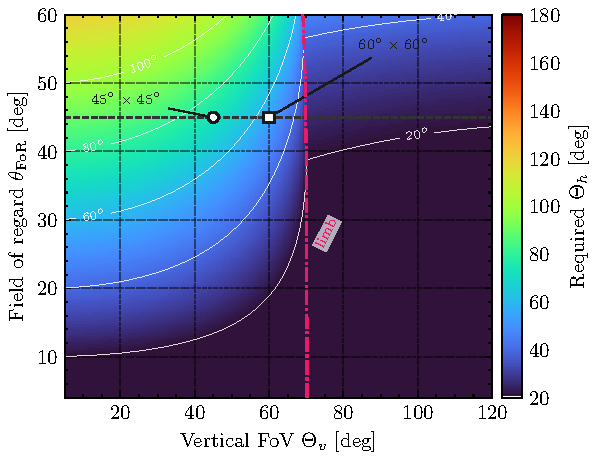
\includegraphics[width=\linewidth]{figures/horizontal_fov_design_map.pdf}
        \caption{Nadir FoR.}
        \label{fig:horizontal_fov_design_map_nadir}
    \end{subfigure}
    \hfill
    \begin{subfigure}[t]{0.49\linewidth}
        \centering
        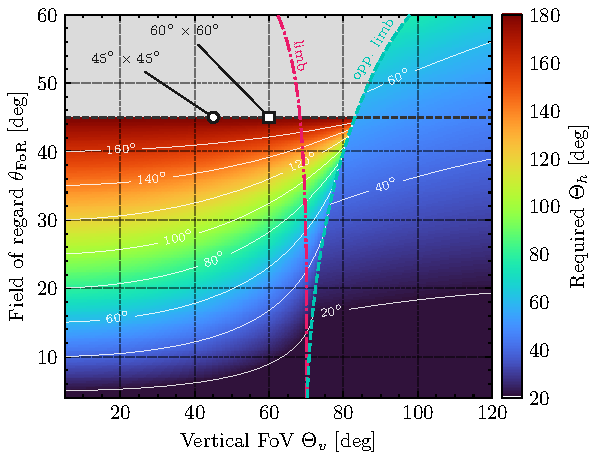
\includegraphics[width=\linewidth]{figures/rolled_body_fov_design_map.pdf}
        \caption{Rolled body, $\varphi=\theta_{\mathrm{FoR}}$.}
        \label{fig:horizontal_fov_design_map_rolled}
    \end{subfigure}
    \caption{Horizontal-FoV requirements induced by vertical FoV and field of regard at $h=\SI{400}{\kilo\metre}$. Heatmaps and contours show the minimum full horizontal FoV; the left panel uses the nadir-FoR requirement in~\eqref{eq:horizontal_fov_requirement}, while the right panel uses the rolled-body contact requirement in~\eqref{eq:rolled_body_horizontal_requirement}. The magenta dash-dotted curves mark where the limb first enters the corresponding detector/FoR geometry; the cyan dashed curve in the rolled panel marks when the opposite FoR edge reaches the detector at the horizon. In the rolled panel, the hatched region has no front-facing contact with both FoR edges inside the rectangular vertical detector band. The dashed line marks the $\pm$\ang{45} primary-imager field of regard used in this paper; markers show the representative \ang{45}$\times$\ang{45} and \ang{60}$\times$\ang{60} lookahead configurations.}
    \label{fig:horizontal_fov_design_map}
\end{figure}

\figref{fig:camera_fov_limit_boxes} visualizes these sizing constraints in common focal-plane coordinates.
The detector boxes are drawn on the same exterior $x/f,y/f$ basis in every panel, with the rolled-body row shown in the native rolled camera frame so that the detector centerline remains on the rolled boresight.

\begin{figure}[htbp]
    \centering
    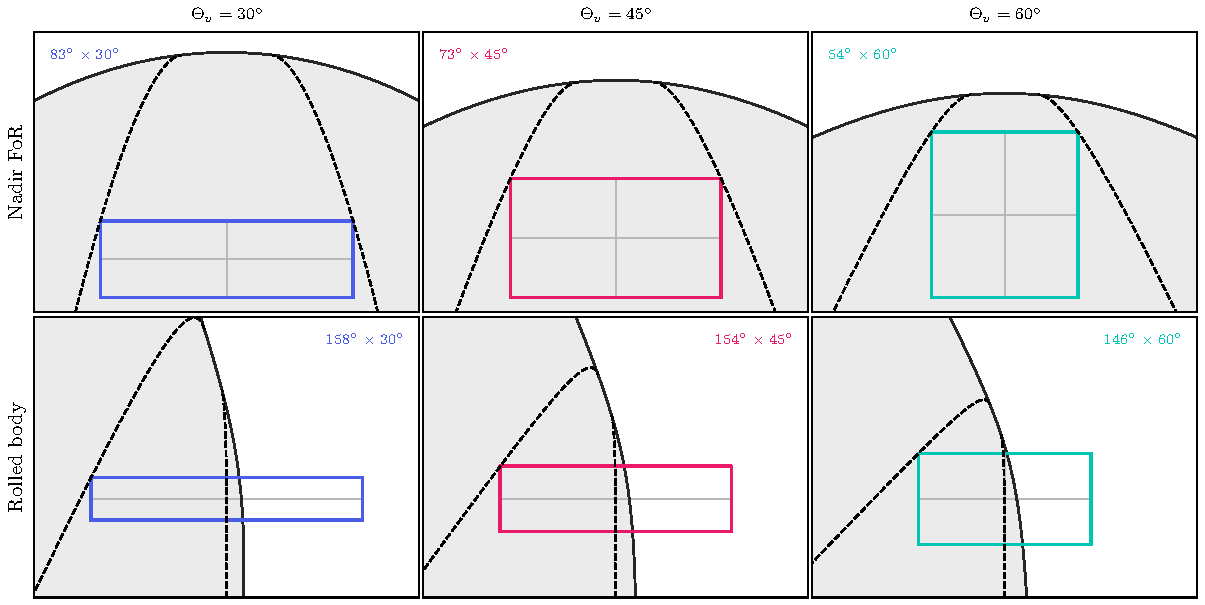
\includegraphics[width=\linewidth]{figures/camera_fov_limit_boxes.pdf}
    \caption{Common-focal camera views of detector boxes at the horizontal-FoV limits for vertical FoVs of \ang{30}, \ang{45}, and \ang{60}. Dashed curves are the field-of-regard envelopes, solid black curves are the horizon limb, shaded regions are Earth, and thin gray lines mark each detector's center axes. Columns vary the vertical FoV; the top row uses the nadir-FoR requirement at $\theta_{\mathrm{FoR}}=\ang{45}$, and the bottom row uses the native rolled-body camera frame at $\theta_{\mathrm{FoR}}=\ang{40}$ to show the near-\ang{180} body-fixed constraint.}
    \label{fig:camera_fov_limit_boxes}
\end{figure}

\paragraph{Instrument configurations.}
\tabref{tab:lookahead_cases} summarizes the two configurations analyzed here. The \emph{stationary} case satisfies the timing and nadir-FoR constraints without re-orientation; the \emph{agile} case sacrifices horizontal coverage and relies on spacecraft re-orientation.

\begin{table}[htbp]
\centering
\caption{Lookahead instrument configurations.}
\label{tab:lookahead_cases}
\begin{tabular}{@{}lccc@{}}
\toprule
\textbf{Case} & \textbf{Vertical FoV} & \textbf{Horizontal FoV} & \textbf{Boresight pitch} \\
\midrule
Stationary & \ang{60} & \ang{60} & \ang{30}   \\
Agile      & \ang{45} & \ang{45} & \ang{22.5} \\
\bottomrule
\end{tabular}
\end{table}

\subsection{Agility Limits}
\label{sec:agility_limits}

The same systems constraints define the limiting behavior of any dynamic-tasking policy.
With instantaneous slew, lookaheads can reveal every scheduled access before execution; if no gap can accommodate a round-trip maneuver, dynamic tasking collapses to the conventional schedule.

\begin{proposition}[Instant-slew omniscience]
\label{prop:omniscience}
Let $J_{\mathrm{omni}}$ denote the optimal MILP utility of~\eqref{eq:scheduling} under realized utilities $u_i = c_i \cdot X_i$ with cloud states $X_i$ revealed. In the limit $t_{\mathrm{slew}} \to 0$, any lookahead policy that observes each scheduled access before its imaging window achieves $J = J_{\mathrm{omni}}$.
\end{proposition}

The proof is given in Appendix~\ref{sec:appendix_proofs}.

\begin{corollary}[Monotonicity in agility]
\label{cor:monotone}
The set of feasible lookahead maneuvers is monotone non-increasing in $t_{\mathrm{slew}}$: any round-trip maneuver feasible at $t_{\mathrm{slew}}'$ is feasible at $t_{\mathrm{slew}} \leq t_{\mathrm{slew}}'$. Consequently, the optimal DT value $J^\star(t_{\mathrm{slew}})$ is non-increasing in $t_{\mathrm{slew}}$, ranging from $J_{\mathrm{omni}}$ at $t_{\mathrm{slew}} = 0$ down to $J_{\mathrm{conv}}$ once no gap admits any round-trip maneuver.
\end{corollary}

\noindent These limits bracket any dynamic-tasking policy without requiring additional simulation.

This system analysis reduces the onboard policy to one candidate lookahead action per schedule gap, searched over a discrete grid of feasible pitch angles.
The remaining question is how to value each candidate angle.

\section{Lookahead Decision Method}
\label{sec:method}

The decision rule is a local mean-field approximation to schedule repair inside a bounded lookahead window.
Its derivation uses four assumptions:
\begin{align}
&\textbf{(A1)}\quad \tau_{ij} \approx g \;\;\forall\,(i,j)\ \text{inside the local repair window}, && \text{constant effective spacing;} \notag\\
&\textbf{(A2)}\quad t_i \overset{\mathrm{i.i.d.}}{\sim} \mathcal{U}(T_1, T_2), && \text{exchangeable access times;} \notag\\
&\textbf{(A3)}\quad X_i \overset{\mathrm{i.i.d.}}{\sim} \mathrm{Bern}(p), && \text{i.i.d.\ cloud states;} \notag\\
&\textbf{(A4)}\quad c_i \approx \bar{c}, && \text{locally equal intrinsic utility.}
\label{eq:assumptions}
\end{align}
Assumption (A1) compresses detailed pairwise slews into the effective dead time used by the chain estimator.
Assumption (A2) is the symmetry exploited by the Poissonization step below: fixed-count uniform access times are equivalent to homogeneous Poisson arrivals conditioned on their count.
Assumptions (A3)--(A4) let the value calculation operate in expected clear-image equivalents; heterogeneous priorities can still enter through the schedule repair MILP after a lookahead is accepted.

\subsection{Two-Anchor Lookahead Value Model}
\label{sec:heuristic}

For a candidate pointing direction at pitch angle $\alpha$ (relative to the boresight rest angle $\alpha_0$), the camera projection determines which not-yet-observed accesses fall within the field of view at the lookahead imaging time.
Only visible accesses no earlier than the next scheduled image are scored, and we denote this set by $\mathcal{V}_\alpha$ with $N_{\mathrm{obs}}(\alpha)=|\mathcal{V}_\alpha|$.
For each schedule gap, the implementation fixes one comparison interval before scoring the pitch grid: $t_L$ is the previous scheduled image (or the planning-window start for the first gap), and $t_R$ is the first scheduled image after the largest feasible detector support over all candidate pitches.
Let
\begin{equation}
L_{\mathrm{anc}} = t_R - t_L
\label{eq:anchor_span}
\end{equation}
be the anchor-to-anchor interval.
All local times below are translated so that the left anchor is at $0$ and the right anchor is at $L_{\mathrm{anc}}$; this same anchor interval is used for every pitch in the gap.
The detector footprint need not span this whole interval.
For pitch $\alpha$, let
\begin{equation}
0 \leq \ell_\alpha < r_\alpha \leq L_{\mathrm{anc}},
\qquad
W_\alpha = r_\alpha-\ell_\alpha
\label{eq:detector_support}
\end{equation}
be the portion of the anchor interval covered by the lookahead detector after applying optimal timing, clipping the near edge at the next scheduled image, and clipping the far edge at the horizon.
Let $N_{\mathrm{sched}}$ be the number of scheduled imaging tasks in the open anchor interval $(t_L,t_R)$ and $N_{\mathrm{missed}}$ the number of scheduled tasks forfeited during the slew.
The net lookahead utility is
\begin{equation}
\widehat{\Delta J} = \underbrace{\hat{J}^+(\mathcal{V}_\alpha)}_{\text{advantage}} - \underbrace{\hat{J}^-(\mathcal{V}_\alpha)}_{\text{opportunity cost}}.
\label{eq:net_advantage}
\end{equation}

\paragraph{Opportunity cost.}
The cost side is local: each forfeited imaging task has expected clear utility $p \cdot \bar{c}$, giving
\begin{equation}
\hat{J}^- = p \cdot \bar{c} \cdot N_{\mathrm{missed}},
\label{eq:opp_cost}
\end{equation}
where $p = P(\text{clear})$ and $\bar{c}$ is the mean intrinsic utility.
The value-based policies below use the timing rule in \secref{sec:timing}, so $N_{\mathrm{missed}}=0$ during normal scoring; the term is retained for calibration windows and for non-optimal timing variants.

\paragraph{Poissonized chain model.}
The advantage side is harder because an observed clear access is valuable only if it can be inserted between the neighboring scheduled images without violating agility constraints.
The schedule anchors define the comparison interval, while the detector support defines where candidate accesses are actually revealed.
Within the clipped detector support, after thinning by the clear-sky prior, the effective clear-candidate density is
\begin{equation}
\lambda_{\mathrm{c}}(\alpha) = \frac{pN_{\mathrm{obs}}(\alpha)}{W_\alpha}.
\label{eq:clear_density}
\end{equation}
The stochastic step exploits the standard symmetry between fixed-count uniform samples and a conditioned Poisson process: conditional on seeing $N_{\mathrm{obs}}$ arrivals in the support interval, the unordered arrival times of a homogeneous Poisson process are i.i.d.\ uniform on that interval~\citep{feller_introduction_1991,david_order_2004}.
Thus the fixed set of visible candidate times can be modeled as a Poisson renewal process conditioned on its count; the onboard approximation then replaces the random clear subset by the unconditioned thinned process with rate $\lambda_{\mathrm{c}}$.
Compressing pairwise slew feasibility into an effective dead time $g$ turns the local repair problem into a one-dimensional packing problem.
With the left and right schedule anchors translated to $0$ and $L_{\mathrm{anc}}$, an insertable clear chain must satisfy
\begin{equation}
t_1 \geq g,\qquad
t_{i+1}-t_i \geq g,\qquad
L_{\mathrm{anc}}-t_k \geq g.
\label{eq:anchored_chain_constraints}
\end{equation}
The two scheduled anchors require one clearance interval at each boundary, but that requirement only removes detector support that lies too close to an anchor.
Define the boundary clearances
\begin{equation}
c_L(\alpha,g)=\max(0,\;g-\ell_\alpha),\qquad
c_R(\alpha,g)=\max(0,\;g-(L_{\mathrm{anc}}-r_\alpha)),
\label{eq:support_clearances}
\end{equation}
and the usable support length
\begin{equation}
U_\alpha(g)=W_\alpha-c_L(\alpha,g)-c_R(\alpha,g).
\label{eq:usable_support}
\end{equation}
After a chain member is accepted, the expected time until the next acceptable clear candidate is the deterministic clearance $g$ plus an exponential waiting time with mean $1/\lambda_{\mathrm{c}}$~\citep{feller_probability_1948,pyke_renewal_1958}.
Thus each additional insertable access consumes, on average,
\begin{equation}
\mathbb{E}[R] = g + \frac{1}{\lambda_{\mathrm{c}}},
\label{eq:renewal_spacing}
\end{equation}
where $R$ is the effective inter-registration spacing of the repaired chain.

For finite windows, the two-anchor chain probability keeps the boundary clearances explicit.
For detector support $[\ell_\alpha,r_\alpha]$ inside the anchor interval and Poisson clear-candidate rate $\lambda_{\mathrm{c}}$, the probability that at least $k$ internal points can be selected with all consecutive gaps at least $g$ is
\begin{equation}
G_\alpha(k;\,g) =
\frac{\gamma\!\big(k,\;\lambda_{\mathrm{c}}\bigl(U_\alpha(g) - (k{-}1)g\bigr)\big)}{\Gamma(k)},
\qquad U_\alpha(g) \geq (k{-}1)g,
\label{eq:chain_prob}
\end{equation}
with $G_\alpha(k;g)=0$ when $U_\alpha(g) < (k{-}1)g$.
The corresponding expected number of insertable internal points is
\begin{equation}
\widehat{K}_{2a}(\alpha,g)
=
\sum_{k\geq 1}
G_\alpha(k;\,g).
\label{eq:chain_expectation}
\end{equation}
When the detector support spans the full anchor interval, $\ell_\alpha=0$ and $r_\alpha=L_{\mathrm{anc}}$, so $c_L=c_R=g$ and~\eqref{eq:chain_prob} reduces to the usual two-boundary form with residual length $L_{\mathrm{anc}}-(k{+}1)g$.
This gives the finite-window advantage score
\begin{equation}
\hat{J}^+_{2a}
=
\bar{c}\,\widehat{K}_{2a}(\alpha,g),
\label{eq:renewal_advantage}
\end{equation}
where the subscript $2a$ denotes the two scheduled anchors.
The exact onboard gate could evaluate $\widehat{K}_{2a}(\alpha,g_{\mathrm{phys}})$ directly; the summation is finite, monotone in $g$, and cheap for the short local windows considered here.

\paragraph{Break-even approximation.}
For a lightweight threshold, we approximate the finite-window chain by its long-run renewal rate on the same usable detector support:
\begin{equation}
\widehat{K}_{b}(\alpha,g)
\;\approx\;
\frac{U_\alpha(g)}{g + 1/\lambda_{\mathrm{c}}(\alpha)}
\;=\;
\frac{\lambda_{\mathrm{c}}(\alpha)U_\alpha(g)}
{1 + \lambda_{\mathrm{c}}(\alpha) g}.
\label{eq:chain_rational_approx}
\end{equation}
This approximation replaces the finite-window chain distribution by its average packing rate.
It has the required behavior for onboard gating: value increases with observed candidate density and decreases monotonically with dead time.
The finite two-anchor form is the higher-fidelity value estimator; $\widehat{K}_{b}$ is the algebraic surrogate that yields a monotone break-even spacing.
Appendix~\ref{sec:appendix_renewal} derives~\eqref{eq:chain_prob} and discusses the residual bias.

\begin{figure}[htbp]
    \centering
    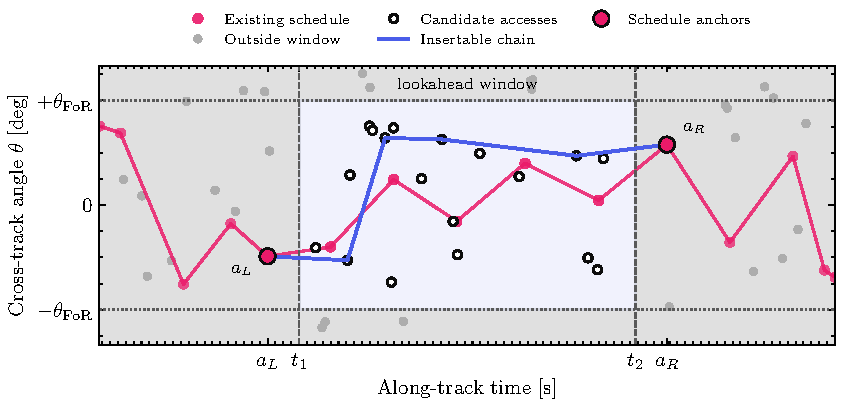
\includegraphics[width=.8\linewidth]{figures/chain_abstraction.pdf}
    \caption{Anchor-bounded lookahead window used by the two-anchor value model. The two scheduled anchors bound the local repair subgraph; gray regions are outside the actionable lookahead window. The model asks whether the expected utility from insertable candidate accesses inside the window exceeds the local replacement burden.}
    \label{fig:chain_abstraction}
\end{figure}

Now write the net advantage in units of average task utility:
\begin{equation}
\frac{\widehat{\Delta J}_{2a}}{\bar{c}}
=
\widehat{K}_{2a}(\alpha,g)
-
\left(p\,N_{\mathrm{sched}} + \frac{\hat{J}^-}{\bar{c}}\right).
\label{eq:normalised_advantage}
\end{equation}
Define the second term as
\begin{equation}
B \;=\; p\,N_{\mathrm{sched}} + \frac{\hat{J}^-}{\bar{c}},
\label{eq:break_even_baseline}
\end{equation}
the number of clear captures that the lookahead must beat: the expected clear captures already present in the local schedule plus any expected opportunity cost from displaced tasks.
Physically, $B$ is the local replacement burden, measured in equivalent unit-clear images.
The first term, $pN_{\mathrm{sched}}$, is the expected number of already-scheduled images in the observation window that the repaired schedule must at least preserve in expectation.
The second term, $\hat{J}^-/\bar{c}$, converts any maneuver-induced loss of scheduled utility into the same units.
Thus $B$ is not a cloud or geometry parameter by itself; it is the number of clear-image equivalents the lookahead must produce before it creates net schedule value.
For pitch search, $B$ is fixed once per schedule gap using the common anchor interval above, while $\mathcal{V}_\alpha$, $W_\alpha$, $\ell_\alpha$, and $r_\alpha$ remain pitch-dependent.
The finite-window gate is therefore $\widehat{K}_{2a}(\alpha,g_{\mathrm{phys}})>B$.
For an onboard engineering threshold, set $\widehat{K}_{b}(\alpha,g_{\mathrm{break}})=B$ using the rational approximation in~\eqref{eq:chain_rational_approx}.
Equivalently,
\begin{equation}
g_{\mathrm{break}}(\alpha)
=
\sup\left\{
g \geq 0:
\frac{\lambda_{\mathrm{c}}(\alpha)U_\alpha(g)}
{1+\lambda_{\mathrm{c}}(\alpha)g}
> B
\right\}.
\label{eq:g_break_alpha}
\end{equation}
If $\lambda_{\mathrm{c}}(\alpha)U_\alpha(0) \leq B$, even a zero-dead-time chain cannot beat the local baseline in this approximation, so the candidate window has no positive break-even spacing.
When the detector support spans the full anchor interval, $\ell_\alpha=0$ and $r_\alpha=L_{\mathrm{anc}}$, \eqref{eq:g_break_alpha} reduces to the closed form
\begin{equation}
g_{\mathrm{break}}
\;\approx\;
\frac{L_{\mathrm{anc}}\left(pN_{\mathrm{obs}} - B\right)}
{pN_{\mathrm{obs}}\left(2+B\right)},
\qquad pN_{\mathrm{obs}} > B.
\label{eq:g_break_full_support}
\end{equation}
Since the packing estimate decreases monotonically with $g$, the lookahead gate can be interpreted as
\begin{equation}
\widehat{\Delta J} > 0
\quad\Longleftrightarrow\quad
g_{\mathrm{phys}} < g_{\mathrm{break}},
\label{eq:break_even_gate}
\end{equation}
up to the approximation in~\eqref{eq:chain_rational_approx}.

This is the key interpretation: $g_{\mathrm{break}}$ is not a replacement for the spacecraft slew time.
It is the maximum effective dead time that the current observation window can tolerate before the expected value of looking falls to zero.
In the common case where opportunity cost is zeroed by optimal timing and the baseline term is dominated by $pN_{\mathrm{sched}}$, this threshold scales with the usable detector support per replacement burden.

The pointing optimization belongs inside this threshold.
For each feasible pitch angle $\alpha$, the camera projection and timing rule induce a different observed-access set, detector support $[\ell_\alpha,r_\alpha]$, and boundary clearances inside the fixed gap-level baseline.
The practical decision variable is therefore the break-even margin
\begin{equation}
M(\alpha)
= g_{\mathrm{break}}(\alpha) - g_{\mathrm{phys}}(\alpha),
\qquad
\alpha^\dagger = \arg\max_{\alpha \in \mathcal{G}_{\alpha}^{\mathrm{feas}}} M(\alpha),
\label{eq:break_even_margin}
\end{equation}
and the lookahead is accepted only when $M(\alpha^\dagger)>0$.
The two-anchor policy reported in the experiments uses the same support and baseline construction but maximizes $\widehat{K}_{2a}(\alpha,g_{\mathrm{phys}})-B$ directly instead of the break-even margin.
For the body-fixed configuration, $g_{\mathrm{phys}}(\alpha)=t_{\mathrm{slew}}(\theta_{\mathrm{FoR}})$ in the chain estimator because the repaired imaging sequence must still tolerate worst-case cross-track slews across the primary imager's field of regard.
The pitch angle $\alpha$ affects the margin through $N_{\mathrm{obs}}(\alpha)$, $W_\alpha$, $\ell_\alpha$, $r_\alpha$, and maneuver feasibility; architectures with angle-dependent imaging dead time can instead substitute their physical $g_{\mathrm{phys}}(\alpha)$ directly into~\eqref{eq:break_even_margin}.

\subsection{Lookahead Sensing Policy: Timing and Pitch}
\label{sec:lookahead_policy}

The value model scores a candidate observation window.
The resulting sensing policy maps the onboard state at a schedule gap to either a lookahead action or the no-look action; if it looks, it must choose when the lookahead occurs and which pitch angle defines the observation window.
Timing is analytic, leaving a one-dimensional pitch search.

\paragraph{Optimal lookahead timing.}
\label{sec:timing}
Let a \emph{schedule gap} $[t_{\mathrm{prev}} + t_s,\; t_{\mathrm{next}}]$ be a maximal idle interval between consecutive imaging tasks.
Timing trades two opposing effects: a later observation sees further into the future and reveals more clear candidates (growing $\hat{J}^+$), but if the round-trip maneuver extends past $t_{\mathrm{next}}$ it begins to displace the next scheduled task (growing $\hat{J}^-$).
The best of both worlds is the latest time at which the maneuver still ends before $t_{\mathrm{next}}$:
\begin{equation}
t^\star(\alpha) = t_{\mathrm{next}} - t_{\mathrm{man}}(\alpha),
\label{eq:optimal_timing}
\end{equation}
where $t_{\mathrm{man}}(\alpha) = 2(t_{\mathrm{slew}}(\alpha - \alpha_0) - t_s)$ is the round-trip maneuver time for pitch angle $\alpha$ and the \emph{actionable} observation window has length
\begin{equation}
L_{\mathrm{act}}(t) = t + t_{\mathrm{horizon}} - t_{\mathrm{next}}.
\label{eq:actionable_window}
\end{equation}

\begin{proposition}[Optimal Lookahead Timing]
\label{prop:timing}
Within a schedule gap, $t = t^\star(\alpha)$ maximizes the net advantage $\widehat{\Delta J}$ up to a bounded perturbation of size $p\bar{c}$, at which point $\hat{J}^- = 0$ and the value gate is evaluated on the clipped detector support inside the fixed gap-level anchor interval.
\end{proposition}

A lookahead at angle $\alpha$ is feasible only if the gap accommodates the maneuver: $t_{\mathrm{next}} - t_{\mathrm{prev}} - t_s \geq t_{\mathrm{man}}(\alpha)$.
The formal proof, including the bounded-perturbation bookkeeping at scheduled-access entries, is given in Appendix~\ref{sec:appendix_proofs}.

\paragraph{Break-even pointing search.}
\label{sec:joint_opt}
Since $t^\star$ depends on $\alpha$, pitch trades access count against maneuver time: steeper pitch observes more accesses but shrinks the actionable window.
The break-even rule evaluates~\eqref{eq:g_break_alpha} over a discrete grid of feasible angles and accepts a lookahead when the best margin in~\eqref{eq:break_even_margin} is positive.
The pitch dependence enters through both the visible-access count and the clipped detector support, while the replacement baseline is held fixed across the pitch grid for that schedule gap.
The implemented policy takes the sensing action $\alpha^\dagger$ from~\eqref{eq:break_even_margin} if $M(\alpha^\dagger)>0$, and takes the no-look action otherwise.

\subsection{Schedule Repair}
\label{sec:schedule_repair}

Once the policy chooses a positive-value lookahead, the spacecraft executes the maneuver, observes the visible accesses, and repairs only the affected schedule segment.
The repair uses receding-horizon re-optimization~\cite{boerkoel_efficient_2021}, treating the lookahead as a schedule-level action gated by the heuristic~\cite{nag_autonomous_2019, augenstein_optimal_2016}.
The spacecraft maintains both a pre-optimized schedule and a priority queue of alternate accesses.
The repair operates on a local subgraph bounded by the nearest scheduled tasks before and after the observation window, which are forced into the MILP to anchor the repaired segment back to the original schedule.
Observed-cloudy accesses are removed from the candidate set; observed-clear and unobserved accesses remain available, with unobserved accesses retaining their prior expected utility $p \cdot c_i$.
The repaired segment is spliced back into the full schedule, and the spacecraft advances to the next imaging block.

Algorithm~\ref{alg:dt_loop} summarizes the full onboard control loop.

\begin{algorithm}[htbp]
\caption{Dynamic tasking control loop}
\label{alg:dt_loop}
\begin{algorithmic}[1]
\Require initial schedule $\boldsymbol{\sigma}_0$, alternates queue $\mathcal{A}_{\text{alt}}$, angle grid $\mathcal{G}_\alpha$, cloud prior $p$
\State $\boldsymbol{\sigma} \gets \boldsymbol{\sigma}_0$
\For{each schedule gap $[t_{\mathrm{prev}}+t_s,\, t_{\mathrm{next}}]$ in $\boldsymbol{\sigma}$}
    \State $\alpha^\dagger \gets \arg\max_{\alpha \in \mathcal{G}_\alpha^{\mathrm{feas}}} M(\alpha)$ \Comment{break-even margin in~\eqref{eq:break_even_margin}}
    \If{$M(\alpha^\dagger) > 0$ \textbf{and} $t_{\mathrm{next}} - t_{\mathrm{prev}} - t_s \geq t_{\mathrm{man}}(\alpha^\dagger)$}
        \State at $t^\star(\alpha^\dagger) = t_{\mathrm{next}} - t_{\mathrm{man}}(\alpha^\dagger)$: slew to $\alpha^\dagger$, observe, slew back \Comment{Prop.~\ref{prop:timing}}
        \State update $\{X_i\}$ for accesses in the observed window
        \State $\boldsymbol{\sigma} \gets \textsc{MILP-Repair}(\boldsymbol{\sigma},\, \mathcal{A}_{\text{alt}},\, \text{bounding accesses})$
    \EndIf
    \State execute scheduled imaging in $[t_{\mathrm{prev}}, t_{\mathrm{next}}]$
\EndFor
\end{algorithmic}
\end{algorithm}

\section{Experiments}
\label{sec:experiments}

\subsection{Experiment Setup}
\label{sec:experiment_setup}

All experiments use a common pool of \num{10000} geographically distributed imaging requests sampled from populated places worldwide.
\figref{fig:worldcities_requests} shows the request distribution.
Each scheduling instance uses a \SI{24}{\hour} planning window and a circular \SI{400}{\kilo\metre} low-Earth orbit with the lookahead instrument configurations from \tabref{tab:lookahead_cases}.
Candidate lookahead observations are evaluated at their imaging time, so cloud state and insertion feasibility are tied to the actual acquisition epoch rather than to access-generation time.
Unless otherwise stated, the realistic-cloud experiments use the BCM clear probability prior $p=0.34$.

\begin{figure}[htbp]
    \centering
    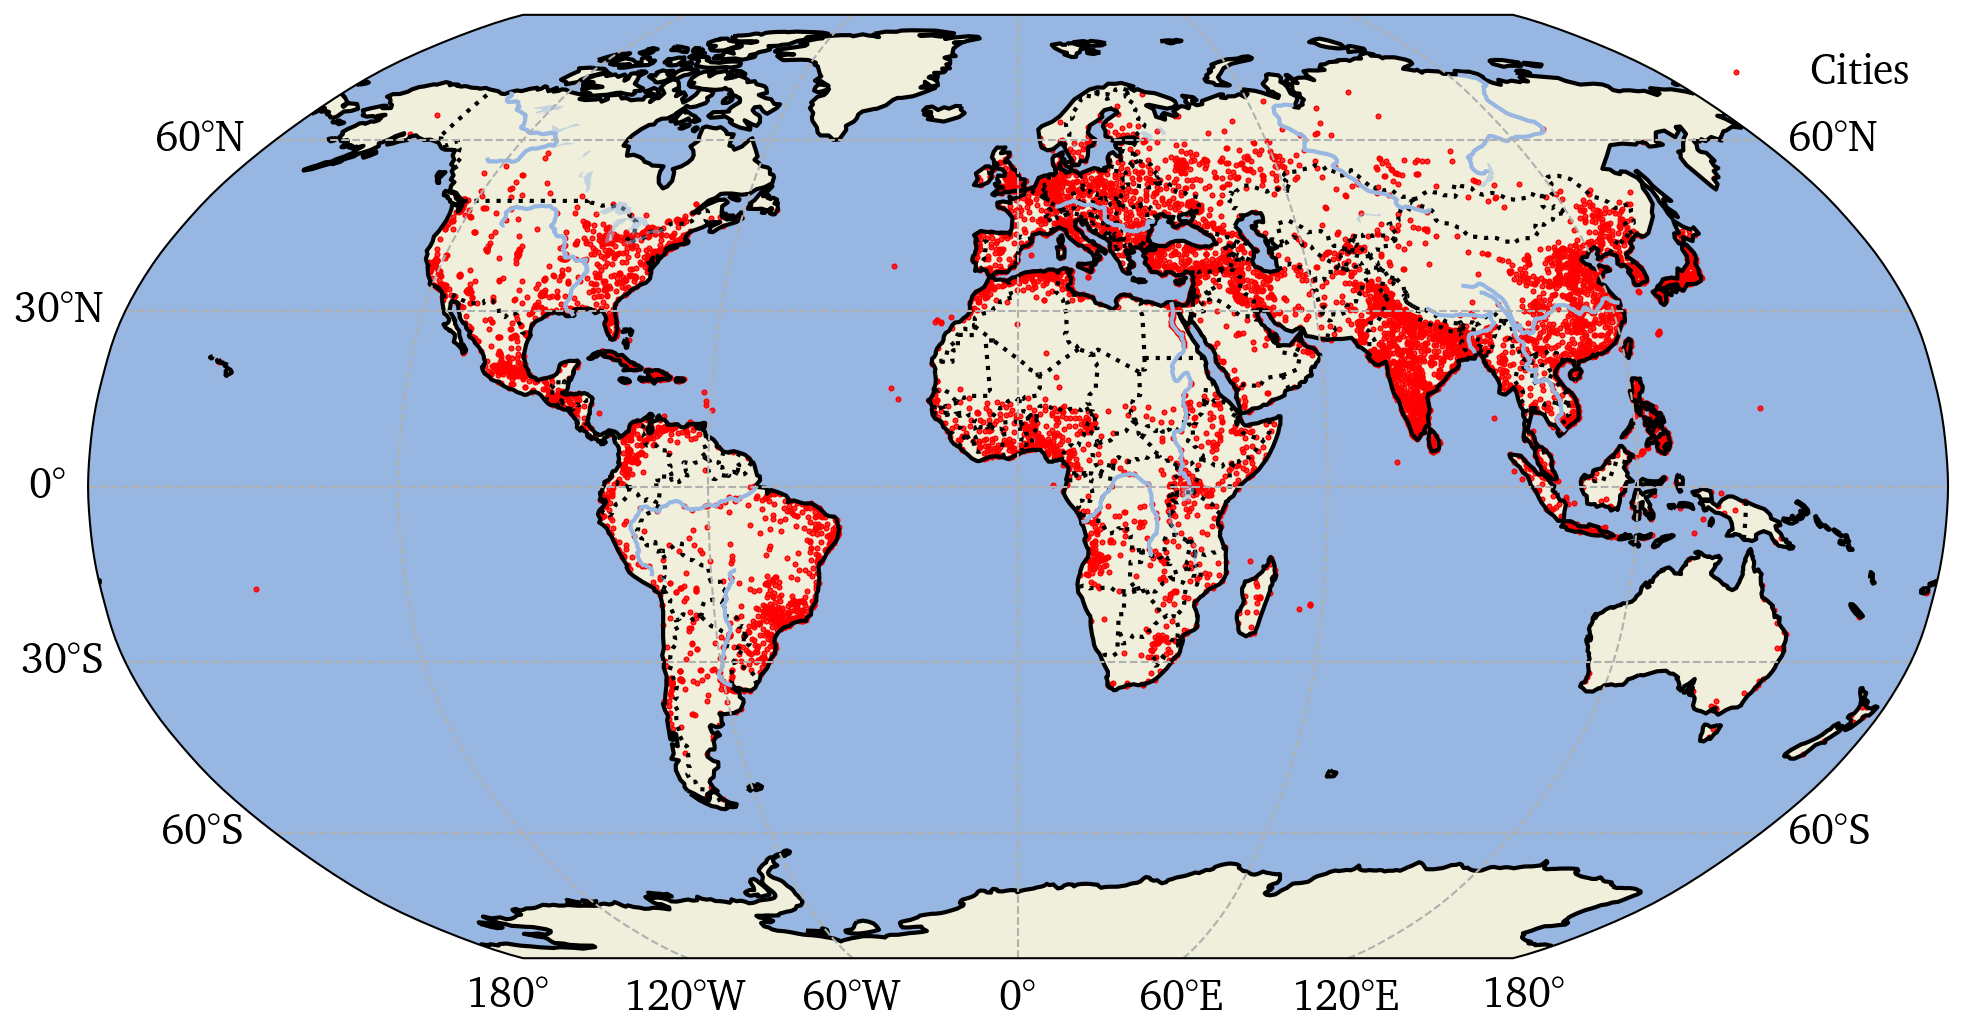
\includegraphics[width=0.72\linewidth]{figures/10k_worldcities.png}
    \caption{Global request set used for the scheduling experiments. The \num{10000} candidate targets are sampled from populated places, yielding dense coverage over major urban corridors while preserving worldwide geographic diversity.}
    \label{fig:worldcities_requests}
\end{figure}

\subsection{Experiment 1: Heuristic Calibration}
\label{sec:exp_heuristic_calibration}

This experiment calibrates the two-anchor value estimate and its break-even surrogate against paired Monte Carlo estimates of the true local insertion advantage in sampled iid repair windows.
The calibration separates the finite-window two-anchor value estimate $\widehat{K}_{2a}(g_{\mathrm{phys}})-B$ from its lightweight break-even surrogate $\widehat{K}_{b}(g_{\mathrm{phys}})-B$; $g_{\mathrm{break}}$ and $M=g_{\mathrm{break}}-g_{\mathrm{phys}}$ are retained as gate diagnostics rather than advantage estimators.
The sampler draws candidate density, cloud probability, physical spacing, and missed-task burden without conditioning on the sign of the heuristic, so the calibration includes both net-positive and net-negative lookahead windows.
For each sampled window, the Monte Carlo value is a conditional expectation over iid Bernoulli cloud states at the fixed candidate access times, not a full orbit-and-weather simulation.
In this iid setting the baseline term $B=p(N_{\mathrm{sched}}+N_{\mathrm{missed}})$ is unbiased by construction, so the residual bias after baseline subtraction reflects the chain approximation rather than the replacement-burden term.
The finite-window two-anchor estimator in \secref{sec:heuristic} removes this dominant boundary effect, while the break-even surrogate remains useful as a lightweight monotone onboard gate.
On the same anchor-normalized windows, the two-anchor advantage estimate attains CCC $0.992$ with bias $-0.025$, compared with CCC $0.982$ and bias $-0.305$ for the break-even surrogate.
All calibration panels report \SI{95}{\percent} bootstrap confidence intervals for CCC and bias, resampling windows while propagating the pointwise Monte Carlo standard error of each conditional mean; shaded bands show the corresponding \SI{95}{\percent} bootstrap confidence intervals for the least-squares calibration line.

\begin{figure}[htbp]
    \centering
    \begin{subfigure}[t]{0.48\linewidth}
        \centering
        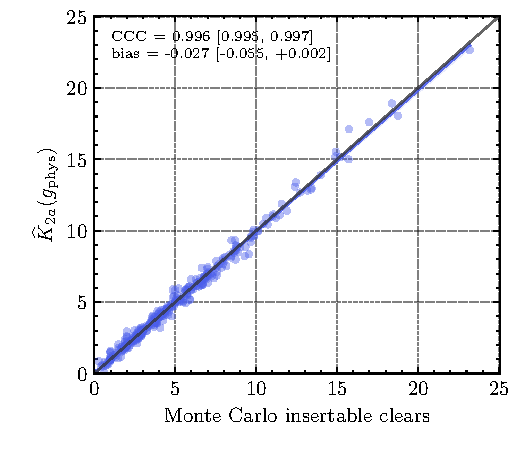
\includegraphics[width=\linewidth]{figures/two_anchor_calibration_chain.pdf}
        \caption{Two-anchor insertable clear-access count.}
        \label{fig:two_anchor_calibration_chain}
    \end{subfigure}
    \hfill
    \begin{subfigure}[t]{0.48\linewidth}
        \centering
        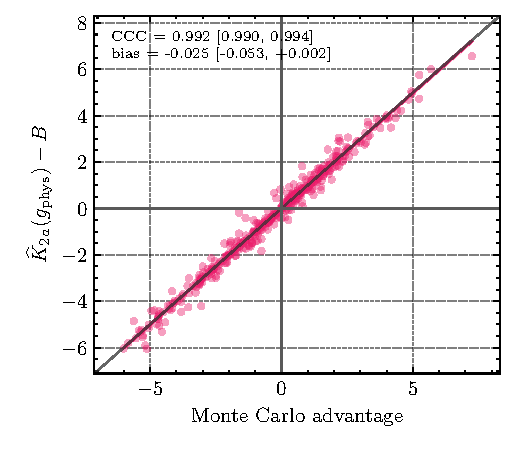
\includegraphics[width=\linewidth]{figures/two_anchor_calibration_advantage.pdf}
        \caption{Two-anchor net advantage.}
        \label{fig:two_anchor_calibration_advantage}
    \end{subfigure}
    \vspace{0.75em}
    \begin{subfigure}[t]{0.48\linewidth}
        \centering
        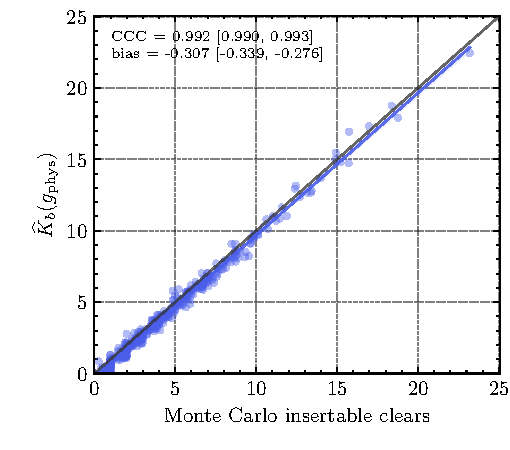
\includegraphics[width=\linewidth]{figures/breakeven_calibration_chain.pdf}
        \caption{Break-even insertable clear-access count.}
        \label{fig:breakeven_calibration_chain}
    \end{subfigure}
    \hfill
    \begin{subfigure}[t]{0.48\linewidth}
        \centering
        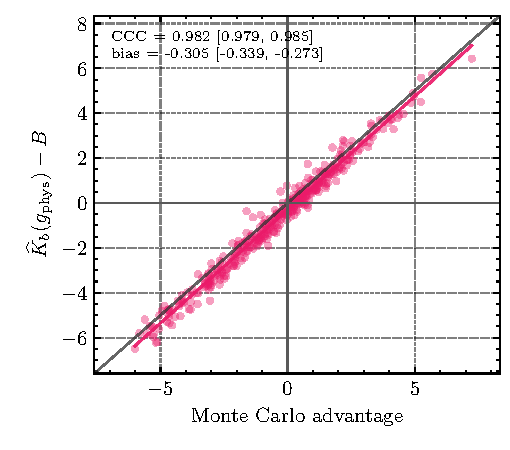
\includegraphics[width=\linewidth]{figures/breakeven_calibration_advantage.pdf}
        \caption{Break-even net advantage.}
        \label{fig:breakeven_calibration_advantage}
    \end{subfigure}
    \caption{Experiment~1 calibration on sampled iid repair windows. Each point fixes one synthetic window and reports the Monte Carlo mean over iid cloud-state draws. Panels compare the two-anchor estimate $\widehat{K}_{2a}(g_{\mathrm{phys}})$ and advantage $\widehat{K}_{2a}(g_{\mathrm{phys}})-B$ against the lightweight break-even surrogate $\widehat{K}_{b}(g_{\mathrm{phys}})$ and $\widehat{K}_{b}(g_{\mathrm{phys}})-B$.}
    \label{fig:heuristic_calibration_2x2}
\end{figure}

\begin{figure}[htbp]
    \centering
    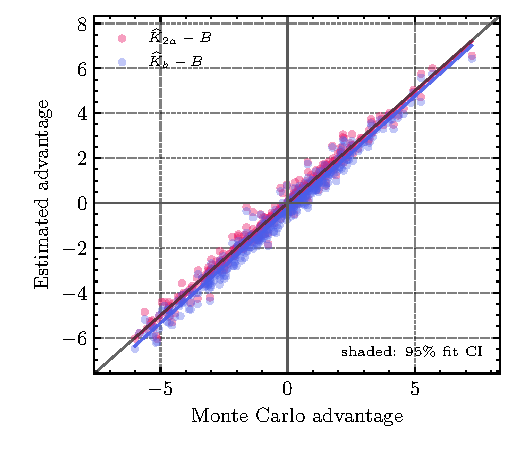
\includegraphics[width=0.5\linewidth]{figures/two_anchor_advantage_comparison.pdf}
    \caption{Direct comparison of the Experiment~1 advantage estimators. Candidate accesses are sampled on the full anchor interval $[t_L,t_R]$, while insertable clear chains must lie in the anchor-trimmed interval $[t_L+g,t_R-g]$. The two-anchor estimator closely tracks the Monte Carlo advantage, whereas the break-even surrogate $\widehat{K}_{b}$ is deliberately lightweight and slightly conservative on these windows. Shaded bands show \SI{95}{\percent} bootstrap confidence intervals for the least-squares calibration lines, including pointwise Monte Carlo standard error.}
    \label{fig:two_anchor_advantage_comparison}
\end{figure}
\FloatBarrier

\subsection{Experiment 2: IID End-to-End Scheduling}
\label{sec:exp_iid_scheduling}

This experiment evaluates greedy, break-even, and two-anchor policies inside the full receding-horizon scheduler under iid Bernoulli cloud truth.
Each trial constructs the conventional schedule, samples realized cloud states independently with $p_{\mathrm{clear}}=0.34$, computes an omniscient clear-sky upper bound, and then replays paired dynamic-tasking policies on the same access set and cloud realization.
To isolate the cloud model, the trial dates and RAAN phase matching are identical to the BCM case study in \secref{sec:exp_bcm_case_study}; only the cloud-state generator changes.
Across \num{12} paired \SI{24}{\hour} trials using the full \num{10000}-request pool, we sweep the two lookahead FoVs in \tabref{tab:lookahead_cases}, $\Theta_h=\Theta_v\in\{\ang{45},\ang{60}\}$, and three representative agility settings, $t_{\mathrm{slew}}(\theta_{\mathrm{FoR}})\in\{25,35,45\}$~s.
Each policy scores \num{64} candidate pitch angles per scheduling gap.
The two-anchor policy tests the finite-window estimator directly, while the break-even policy tests the monotone gate derived from $\widehat{K}_{b}$.
Across all FoV/agility cells, the value-based policies dominate the greedy baseline in gap closure while using about \SI{40}{\percent} fewer lookahead actions per scheduled access.
Averaged across the sweep, greedy closes \SI{51.3}{\percent} of the omniscient gap with 0.270 lookaheads per scheduled access.
The break-even gate closes \SI{72.1}{\percent} with 0.163 lookaheads per scheduled access, while the two-anchor policy closes \SI{72.8}{\percent} with 0.166.
The strongest cell is the \ang{60}$\times$\ang{60} lookahead FoV with $t_{\mathrm{slew}}(\theta_{\mathrm{FoR}})=\SI{45}{\second}$: break-even closes \SI{82.1}{\percent} of the gap with 0.200 lookaheads per scheduled access, and two-anchor closes \SI{81.9}{\percent} with 0.200.
\todo{Expand this interpretation: break-even and two-anchor are nearly indistinguishable in the iid end-to-end scheduler once the anchor-support correction is applied, so the final paper should decide whether to present break-even as the lightweight onboard rule and two-anchor as its finite-window justification.}
Detailed numerical summaries are reported in Appendix~\ref{sec:appendix_iid_scheduling_summary}.

\begin{figure}[H]
    \centering
    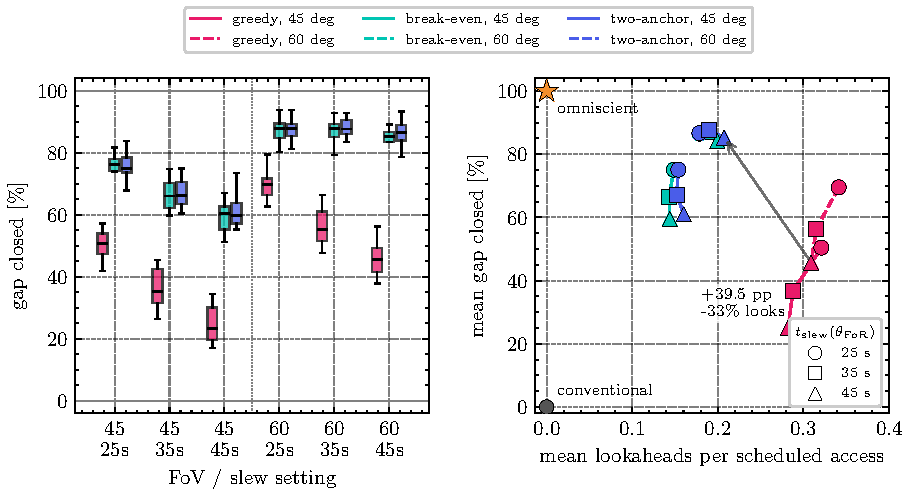
\includegraphics[width=0.92\linewidth]{figures/iid_scheduling_tradeoff.pdf}
    \caption{IID end-to-end scheduling over \num{12} paired \SI{24}{\hour} trials per FoV/agility cell. Left: per-trial distribution of the conventional-to-omniscient gap fraction closed. Right: mean gap closure versus mean lookaheads per scheduled access for the same FoV/agility cells; marker shape encodes agility. Solid lines use the \ang{45}$\times$\ang{45} lookahead FoV; dashed lines use the \ang{60}$\times$\ang{60} FoV. The gray dot and orange star mark the conventional and omniscient references.}
    \label{fig:iid_scheduling_tradeoff}
\end{figure}

\subsection{Experiment 3: Realistic BCM Case Study}
\label{sec:exp_bcm_case_study}

This experiment repeats the end-to-end scheduler sweep using realistic cloud truth from geostationary Binary Cloud Mask products.
We use \num{12} paired \SI{24}{\hour} windows spanning the available 2025 archive, with trial starts on Jan.~1, Feb.~2, Mar.~1, Apr.~1, May~1, Jun.~1, Jul.~1, Aug.~1, Sep.~1, Oct.~1, Oct.~10, and Dec.~1.
The February and late-year dates are shifted from exact month starts only to avoid verified source-product gaps in the GOES and Himawari archives.
For all date-based trials, the RAAN is phase-matched to the first window so that each trial repeats the same Earth-fixed ground track; remaining seasonal variation therefore comes from illumination and cloud structure rather than from a drifting target overpass pattern.
The policy prior remains fixed at $p_{\mathrm{clear}}=0.34$, while realized clear/cloudy states are sampled from the nearest available source product at each access imaging time.

\figref{fig:bcm_scheduling_tradeoff} shows that the value-based gates remain effective under spatially structured cloud fields.
Averaged across all six FoV/agility cells, the break-even gate closes \SI{70.1}{\percent} of the conventional-to-omniscient gap using 0.162 lookaheads per scheduled access, while the two-anchor gate closes \SI{71.8}{\percent} using 0.165 lookaheads per scheduled access.
The greedy baseline closes \SI{36.7}{\percent} on average but uses 0.264 lookaheads per scheduled access.
The strongest BCM setting is the \ang{60}$\times$\ang{60} lookahead FoV with $t_{\mathrm{slew}}(\theta_{\mathrm{FoR}})=\SI{45}{\second}$: break-even closes \SI{80.1}{\percent} of the gap with 0.196 lookaheads per scheduled access, and two-anchor closes \SI{81.3}{\percent} with 0.198.
With the anchor-consistent support definition, the two-anchor estimator and break-even surrogate now make similar operational decisions; two-anchor is slightly stronger on average in this sweep.
Detailed numerical summaries are reported in Appendix~\ref{sec:appendix_bcm_scheduling_summary}.

\begin{figure}[H]
    \centering
    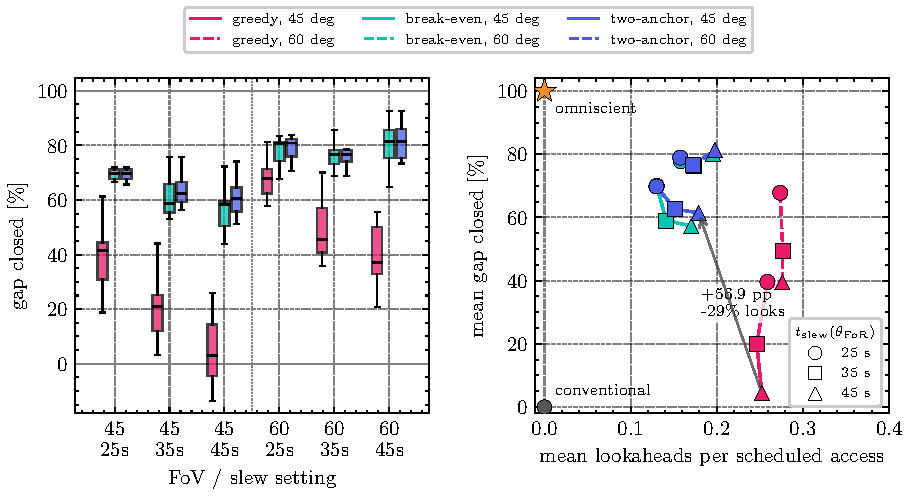
\includegraphics[width=0.92\linewidth]{figures/bcm_scheduling_tradeoff.pdf}
    \caption{BCM end-to-end scheduling over \num{12} paired \SI{24}{\hour} trials per FoV/agility cell. Trial RAAN is phase-matched across dates to preserve the Earth-fixed ground track while cloud truth is sampled from realistic geostationary cloud-mask products at each access imaging time. Left: per-trial distribution of the conventional-to-omniscient gap fraction closed. Right: mean gap closure versus mean lookaheads per scheduled access; marker shape encodes agility, line style encodes FoV, and the gray dot/orange star mark conventional and omniscient references.}
    \label{fig:bcm_scheduling_tradeoff}
\end{figure}

\subsection{Experiment 4: Overflight Case Study}
\label{sec:exp_overflight_case_study}

As a representative single-pass case study, \figref{fig:ma_overflight_case_study} compares the two value-based policies on the same Morocco-to-Australia overflight and iid cloud realization.
Both panels use the same access set, conventional schedule, and camera model; only the lookahead gate changes.
Break-even uses \num{11} lookaheads and two-anchor uses \num{14}, with both policies scheduling \num{48} clear images after local repair.

\begin{figure}[H]
    \centering
    \begin{subfigure}[t]{0.48\linewidth}
        \centering
        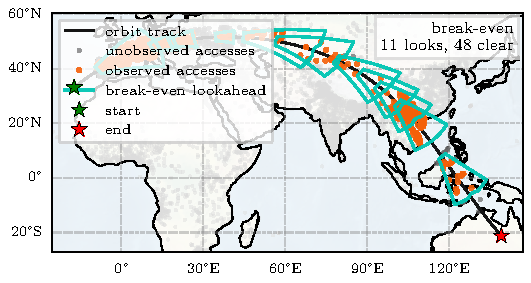
\includegraphics[width=\linewidth]{figures/lookahead_chain_ma_break_even.pdf}
        \caption{Break-even gate.}
        \label{fig:ma_overflight_break_even}
    \end{subfigure}
    \hfill
    \begin{subfigure}[t]{0.48\linewidth}
        \centering
        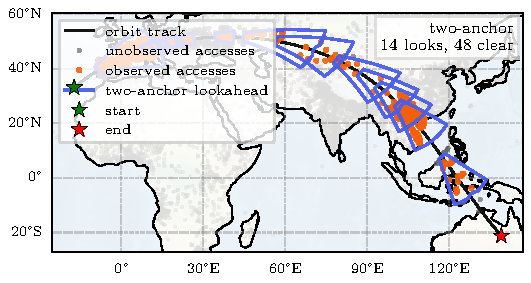
\includegraphics[width=\linewidth]{figures/lookahead_chain_ma_two_anchor.pdf}
        \caption{Two-anchor gate.}
        \label{fig:ma_overflight_two_anchor}
    \end{subfigure}
    \caption{Representative Morocco-to-Australia overflight case study. Orange dots mark accesses observed by the lookahead instrument, gray dots mark unobserved accesses, and colored outlines show the detector footprints selected by each policy.}
    \label{fig:ma_overflight_case_study}
\end{figure}

\figref{fig:brazil_overflight_case_study} shows the same comparison on the South America overpass used during development.
This case includes a zero-utility virtual anchor near the start of the pass so that the receding-horizon rule can evaluate the initial offshore reconnaissance gap before the first conventional imaging task.
With that anchor, both value gates take \num{6} lookaheads and schedule \num{23} clear images in the repaired pass.

\begin{figure}[H]
    \centering
    \begin{subfigure}[t]{0.48\linewidth}
        \centering
        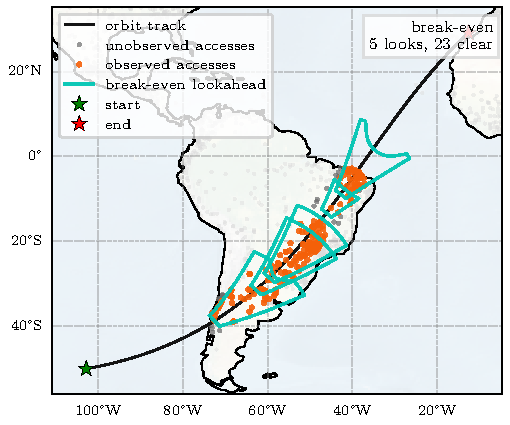
\includegraphics[width=\linewidth]{figures/lookahead_chain_brazil_break_even.pdf}
        \caption{Break-even gate.}
        \label{fig:brazil_overflight_break_even}
    \end{subfigure}
    \hfill
    \begin{subfigure}[t]{0.48\linewidth}
        \centering
        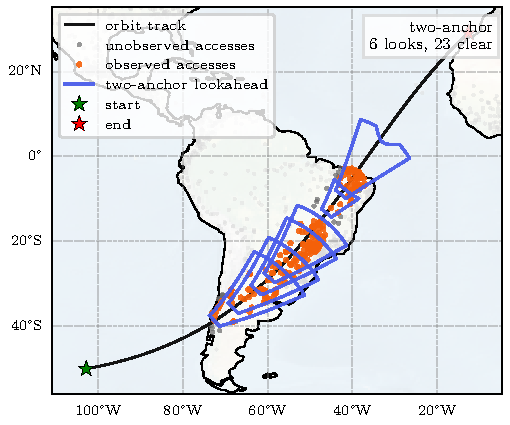
\includegraphics[width=\linewidth]{figures/lookahead_chain_brazil_two_anchor.pdf}
        \caption{Two-anchor gate.}
        \label{fig:brazil_overflight_two_anchor}
    \end{subfigure}
    \caption{Brazil overpass case study using the same visual encoding as \figref{fig:ma_overflight_case_study}.}
    \label{fig:brazil_overflight_case_study}
\end{figure}

\section{Conclusion}
\label{sec:conclusion}

We derive a two-boundary renewal estimator for deciding when a body-fixed lookahead maneuver is worth its schedule cost, then reduce it to a monotone break-even heuristic for lightweight onboard gating.
The estimator separates the physical slew prior from a schedule-dependent break-even spacing, and the optimal-timing result (Proposition~\ref{prop:timing}) collapses the one-dimensional timing search to a closed-form initiation time that incurs zero opportunity cost up to a bounded perturbation.
Together, the break-even margin, timing rule, and pitch search produce an onboard policy that asks a direct engineering question: whether any feasible pointing angle can generate enough expected clear-image equivalents to beat the local replacement burden.

\paragraph{Limitations.}
The policy's value estimator assumes equal task utility (A4), i.i.d.\ cloud states (A3), and constant gap spacing (A1).
Relaxing these---particularly for heterogeneous Pareto-distributed task values---is necessary for realistic commercial operations where a small fraction of high-value tasks dominates schedule utility.
The analysis also assumes perfect lookahead classification once an access is visible.
False positives would insert cloudy tasks into the repaired schedule, while false negatives would suppress useful alternate accesses; quantifying sensitivity to classifier precision and recall is therefore necessary before mapping the method to a specific onboard vision pipeline.

\paragraph{Future work.}
Extending the chain-length analysis to utility-weighted chains would address the Pareto case.
Multi-step lookaheads within a single gap could improve coverage for narrow-FoV instruments.
Constellation extensions with shared belief states across spacecraft could reduce redundant observations, and pre-planning lookahead opportunities in the ground schedule could yield global improvements at the cost of additional computational complexity.


\FloatBarrier
\bibliographystyle{unsrtnat}
\bibliography{references}

\appendix

\section{Supporting System Data}
\label{sec:appendix_system_data}

\begin{table}[htbp]
\centering
\caption{Agility specifications for representative tasked EO satellites, scaled to a \ang{90} slew.}
\label{tab:agility}
\sisetup{table-format=2.1}
\begin{tabular}{@{}l c c l S@{}}
\toprule
\textbf{Platform} & \textbf{Launch} & \textbf{FoR} & \textbf{Manufacturer spec} & {\textbf{Scaled \ang{90} slew [s]}} \\
\midrule
WorldView-1~\citep{maxar_technologies_worldview-1_nodate} & 2007 & $\pm\ang{45}$ & \SI{2.5}{\degree/\second^2},\ \SI{4.5}{\degree/\second}\ max & 24.7 \\
Pl{\'e}iades 1A/1B~\citep{amram_pleiades_nodate}          & 2011 & $\pm\ang{47}$ & \ang{60} in \SI{25}{\second} (incl.\ settle)                 & 37.5 \\
SPOT-6~\citep{noauthor_spot6_nodate}                      & 2012 & $\pm\ang{45}$ & \ang{30} in \SI{14}{\second}                                 & 42.0 \\
Pl{\'e}iades Neo~\citep{noauthor_pleiades_nodate}         & 2022 & $\pm\ang{47}$ & \ang{60} in \SI{20}{\second}                                 & 30.0 \\
\bottomrule
\end{tabular}
\end{table}

\section{Proofs and Derivations}
\label{sec:appendix_proofs}

\subsection{FoR-Edge Projection}
\label{sec:appendix_fov_projection}

The nadir and rolled horizontal-FoV constraints use the same rectilinear projection of a primary-imager FoR edge.
Let $a=R_E+h$, $\beta=\Theta_v/2$, $\rho_F=\rho(\theta_{\mathrm{FoR}})$, $R_F=\sqrt{R_E^2-\rho_F^2}$, and let $\sigma\in\{-1,+1\}$ index the two FoR edges, with $F$ denoting the fixed FoR-edge slice.
Use the same local frame as \figref{fig:lookahead_geometry}: $x$ is the forward local-horizontal projection from $N$, $\sigma\rho_F$ is the cross-track local-horizontal projection of the FoR edge, and $z(x)$ is the component from $S$ toward Earth along the nadir line $SN$.
For a point on either FoR edge, that nadir-axis depth and the forward limb coordinate are
\begin{equation}
z(x)=a-\sqrt{R_F^2-x^2},
\qquad
x_{\mathrm{limb}}=\sqrt{R_E^2\left(1-\left[\frac{R_E}{a}\right]^2\right)-\rho_F^2}.
\label{eq:rolled_body_ray}
\end{equation}
For body roll $\varphi$, the detector-plane horizontal offset, vertical offset, and boresight depth are
\begin{equation}
\begin{aligned}
\delta_\sigma(x;\varphi)
&=\sigma\rho_F\cos\varphi-z(x)\sin\varphi,\\
\eta_\sigma(x;\varphi)
&=x\cos\beta-\sin\beta\left[z(x)\cos\varphi+\sigma\rho_F\sin\varphi\right],\\
d_\sigma(x;\varphi)
&=x\sin\beta+\cos\beta\left[z(x)\cos\varphi+\sigma\rho_F\sin\varphi\right].
\end{aligned}
\label{eq:rolled_body_depth_offset}
\end{equation}
The rectangular-detector condition is
\begin{equation}
\mathcal{D}_\sigma(\varphi) =
\left\{x\in[0,x_{\mathrm{limb}}]\;:\;
\left|\eta_\sigma(x;\varphi)\right|\leq d_\sigma(x;\varphi)\tan\beta,\;
d_\sigma(x;\varphi)>0\right\},
\label{eq:rolled_vertical_band}
\end{equation}
and the horizontal look angle is
\begin{equation}
\lambda_\sigma(x;\varphi)=
\operatorname{atan2}\!\left(\delta_\sigma(x;\varphi),d_\sigma(x;\varphi)\right).
\label{eq:rolled_horizontal_angle}
\end{equation}
The key point is that this is a flat focal-plane condition; replacing it with a viewing-sphere latitude bound describes a different detector.

\subsection{Nadir-FoR Limiting Point}
\label{sec:appendix_nadir_fov}

The nadir-FoR requirement in~\eqref{eq:horizontal_fov_requirement} is the $\varphi=0$ specialization of the FoR-edge projection.
The limiting point lies on a FoR edge with cross-track coordinate $\rho_F$.
With $a=R_E+h$ and $\beta=\Theta_v/2$, the upper detector edge is the rectilinear condition
\begin{equation}
\frac{x\cos\beta-z\sin\beta}
{x\sin\beta+z\cos\beta}
=\tan\beta
\quad\Longleftrightarrow\quad
\frac{x}{z}=\tan\Theta_v.
\label{eq:nadir_upper_edge_condition}
\end{equation}
Combining~\eqref{eq:nadir_upper_edge_condition} with the spherical height relation
$z=a-\sqrt{R_F^2-x^2}$ gives the upper-edge contact
\begin{equation}
x_{\mathrm{edge}} =
\sin\Theta_v
\left[
a\cos\Theta_v
-\sqrt{R_F^2-a^2\sin^2\Theta_v}
\right],
\label{eq:nadir_upper_edge_contact}
\end{equation}
provided the square-root term is real and the upper edge intersects Earth before the limb.
Otherwise the limiting point is the forward limb point on the same FoR edge,
\begin{equation}
x_{\mathrm{limb}} =
\sqrt{
R_E^2\left(1-\left[\frac{R_E}{a}\right]^2\right)-\rho_F^2
}.
\label{eq:nadir_horizon_cap}
\end{equation}
The transition occurs when the upper detector edge first reaches the limb,
\begin{equation}
\Theta_v
=
\arcsin\!\left(\frac{R_F}{a}\right).
\label{eq:nadir_limb_transition}
\end{equation}

\subsection{Rolled-Body FoR Candidate Equations}
\label{sec:appendix_rolled_fov}

The rolled-body requirement in~\eqref{eq:rolled_body_horizontal_requirement} uses the same FoR-edge projection with $\varphi=\theta_{\mathrm{FoR}}$.
Under this roll convention, the same-side FoR point is pinned to the lower detector center and the opposite FoR edge sets the horizontal width.
The upper-edge contact in~\eqref{eq:rolled_opposite_contact} is the admissible root, for $\sigma=-1$, of
\begin{equation}
\eta_\sigma(x;\varphi)=d_\sigma(x;\varphi)\tan\beta.
\label{eq:rolled_vertical_boundary}
\end{equation}
Equivalently, with $z(x)=a-\sqrt{R_F^2-x^2}$,
\begin{equation}
x=\tan(2\beta)
\left[z(x)\cos\varphi+\sigma\rho_F\sin\varphi\right].
\label{eq:rolled_upper_edge_contact}
\end{equation}
With the same shorthand used in the main text,
$Q=\cot(2\beta)$ and $K_\sigma=a\cos\varphi+\sigma\rho_F\sin\varphi$.
Substituting $z(x)=a-\sqrt{R_F^2-x^2}$ into~\eqref{eq:rolled_upper_edge_contact} gives
$Qx=K_\sigma-\cos\varphi\sqrt{R_F^2-x^2}$, so the candidate roots satisfy
\begin{equation}
\left(\cos^2\varphi+Q^2\right)x^2
-2K_\sigma Qx
+K_\sigma^2-\cos^2\varphi\,R_F^2=0.
\label{eq:rolled_upper_edge_quadratic}
\end{equation}
The closed form in~\eqref{eq:rolled_upper_contact_closed_form} follows from this quadratic.
Roots are retained only if they satisfy the unsquared relation
$Qx=K_\sigma-\cos\varphi\sqrt{R_F^2-x^2}$ and the front-facing vertical-band constraint $x\in\mathcal{D}_\sigma(\varphi)$.
For the opposite-edge engineering expression, $x_{\mathrm{upper}}$ is the retained $\sigma=-1$ root that minimizes $\left|\lambda_-(x;\varphi)\right|$.

The fully general implementation evaluates $\left|\lambda_\sigma(x;\varphi)\right|$ on a finite candidate set for both $\sigma\in\{-1,+1\}$ and keeps points satisfying $x\in\mathcal{D}_\sigma(\varphi)$.
This set consists of the interval endpoints $x=0$ and $x=x_{\mathrm{limb}}$, detector-edge contacts from~\eqref{eq:rolled_vertical_boundary}, and interior stationary contacts of
$\lambda_\sigma(x;\varphi)=\operatorname{atan2}(\delta_\sigma(x;\varphi),d_\sigma(x;\varphi))$.
Since
\begin{equation}
\frac{d\lambda_\sigma}{dx}=0
\quad\Longleftrightarrow\quad
d_\sigma(x;\varphi)\delta_\sigma'(x;\varphi)-\delta_\sigma(x;\varphi)d_\sigma'(x;\varphi)=0,
\label{eq:rolled_stationary_condition}
\end{equation}
the stationarity condition can be written compactly as
\begin{equation}
p_\sigma x+q_\sigma\sqrt{R_F^2-x^2}+r=0,
\label{eq:rolled_stationary_compact}
\end{equation}
where
\begin{equation}
p_\sigma=\sigma\rho_F\cos\beta,\qquad
q_\sigma=\sin\beta\left[\sigma\rho_F\cos\varphi-a\sin\varphi\right],
\qquad
r=R_F^2\sin\beta\sin\varphi.
\end{equation}
Squaring~\eqref{eq:rolled_stationary_compact} gives the quadratic candidate equation
\begin{equation}
(p_\sigma^2+q_\sigma^2)x^2
 +2p_\sigma r\,x
 + r^2-q_\sigma^2R_F^2 = 0.
\label{eq:rolled_stationary_quadratic}
\end{equation}
Because squaring can introduce extraneous roots, stationary candidates from~\eqref{eq:rolled_stationary_quadratic} are kept only if they also satisfy the unsquared condition~\eqref{eq:rolled_stationary_compact}.
If no candidate remains for either one of the two FoR edges, the rolled body-fixed configuration is infeasible for that $(\Theta_v,\theta_{\mathrm{FoR}})$ pair.

\subsection{Two-Boundary Renewal Estimator}
\label{sec:appendix_renewal}

This appendix derives the support-aware two-boundary probability in~\eqref{eq:chain_prob} and records the residual bias source for the finite-window estimator used in \secref{sec:heuristic}.
The main text gives the estimator and the break-even surrogate; the derivation below shows why the incomplete-gamma term is the anchored packing probability.

\subsection{Derivation of the Two-Boundary Chain Probability}

Place the two schedule anchors at positions $0$ and $L$, and let the detector reveal clear candidates only on the support interval $[\ell,r]\subseteq[0,L]$.
Consider $k$ internal chain points
\begin{equation}
\ell \leq t_1 < t_2 < \dots < t_k \leq r.
\end{equation}
The anchor spacing constraints are $t_1 \geq g$, $t_{i+1}-t_i \geq g$ for $i=1,\dots,k{-}1$, and $L-t_k \geq g$.
The boundary constraints only remove support that lies too close to the anchors, so define
\begin{equation}
c_L=\max(0,g-\ell),\qquad
c_R=\max(0,g-(L-r)),\qquad
U=(r-\ell)-c_L-c_R.
\end{equation}
After trimming these boundary clearances, the first accepted point can occur at the start of the usable interval, while each additional internal point requires one deterministic clearance $g$ plus one exponential wait.
Under Poissonization~\cite{jacquet_analytical_1998, feller_probability_1948}, the total time needed to place $k$ internal points inside usable support is
\begin{equation}
S_k = (k{-}1)g + \underbrace{\sum_{i=1}^{k} X_i}_{Y_k},
\end{equation}
where $Y_k \sim \Gamma(k, \lambda)$ as a sum of i.i.d.\ exponentials~\cite{feller_introduction_1991}.
Equivalently, the $k$ internal points correspond to $k$ Poisson arrivals falling in the residual interval of length $U-(k{-}1)g$.
By the Poisson--Gamma duality $P(\mathrm{Pois}(\mu) \geq k) = \gamma(k, \mu)/\Gamma(k)$ with $\mu = \lambda\bigl(U-(k{-}1)g\bigr)$, giving~\eqref{eq:chain_prob}.
The shape parameter is $k$ because fitting $k$ internal arrivals requires $k$ exponential waits; the anchor clearances and the $k{-}1$ internal clearances are deterministic.
This corresponds to the \emph{non-paralyzable} (Type~I) counter convention with both ends anchored~\cite{pyke_renewal_1958}.
When $[\ell,r]=[0,L]$, $U=L-2g$ and the residual interval becomes $L-(k{+}1)g$, recovering the standard full-support two-boundary form.

\subsection{Proof of Proposition~\ref{prop:omniscience} (Instant-Slew Omniscience)}

With zero slew time, a lookahead can be inserted immediately before each candidate access at no opportunity cost.
Because onboard observations are assumed noise-free, every cloud state $X_i$ is revealed before the corresponding imaging decision is made.
The scheduler can therefore solve~\eqref{eq:scheduling} with realized utilities $u_i = c_i \cdot X_i$ in place of expected utilities, recovering the omniscient optimum. \qed

\subsection{Proof of Proposition~\ref{prop:timing} (Optimal Lookahead Timing)}

Decompose
$\widehat{\Delta J}(t)/\bar{c}
= E[K;\, \lambda_c(t),\, W(t),\, \ell(t),\, r(t),\, L_{\mathrm{anc}},\, g]
- p\, N_{\mathrm{sched}}(t)
- \hat{J}^-(t)/\bar{c}$,
where $E[K;\cdot]$ is the support-aware two-boundary chain-length estimator from~\eqref{eq:chain_expectation} applied to the clipped detector support $[\ell(t),r(t)]$ inside the fixed anchor interval.
Both $N_{\mathrm{obs}}(t)$ and the support end $r(t)$ are non-decreasing step/continuous functions of $t$: they grow when visible accesses or newly reachable detector support enter the actionable window $[t_{\mathrm{next}},\, t+t_{\mathrm{horizon}}]$.
Between access entries, the chain term is smoothly non-decreasing in the clipped support at fixed $N_{\mathrm{obs}}$.
If the baseline is charged only once per fixed schedule gap, as in the implementation, this monotonicity is direct; if scheduled tasks are charged as they enter the local window, $N_{\mathrm{sched}}(t)$ is a non-decreasing step function and the following bounded-jump argument applies.
At a scheduled-access entry, $p\, N_{\mathrm{sched}}$ jumps up by $p$ while the chain term jumps up by the marginal contribution of one additional candidate (bounded by $p$ since each new candidate is independently clear with probability $p$); the net jump in $\widehat{\Delta J}$ is therefore bounded below by $-p\bar{c}$.
Hence $\widehat{\Delta J}$ is piecewise-smoothly non-decreasing with bounded downward steps of size at most $p\bar{c}$ while $\hat{J}^-=0$.

For $t \leq t^\star(\alpha)$, the maneuver terminates no later than $t_{\mathrm{next}}$, so $\hat{J}^- = 0$ and the net advantage is the finite-window chain value minus the local baseline burden.
For $t > t^\star(\alpha)$, $\hat{J}^-$ steps up by $p\bar{c}$ for each scheduled task whose imaging time falls in the maneuver interval $[t,\, t+t_{\mathrm{man}}(\alpha)]$, which equals or exceeds the concurrent marginal gain of $\hat{J}^+$ so the net advantage is non-increasing past $t^\star(\alpha)$.
Therefore $t^\star(\alpha)$ maximizes $\widehat{\Delta J}$ up to at most one bounded perturbation of size $p\bar{c}$, with equality when no scheduled access enters the observation window within a small left-neighborhood of $t^\star(\alpha)$.
\qed

\section{Bias Analysis Details}
\label{sec:appendix_bias}

The two-boundary form in~\eqref{eq:chain_prob} already absorbs the dominant bias source present in a naive one-anchor renewal estimate: the usable support $U$ explicitly removes only the detector support that violates the left or right anchor clearance, rather than over-counting free space near $0$ and $L$.
The remaining bias is small and of a single sign.

\paragraph{Poissonization variance (residual negative bias).}
Replacing $N$ fixed points with $\mathrm{Poisson}(N)$ introduces count variance.
Since the chain length $f(n)$ is concave in the number of points (diminishing returns), Jensen's inequality gives $\mathbb{E}[f(\mathrm{Poisson}(N))] \leq f(N)$, producing a small negative bias.
A standard de-Poissonization correction~\cite{jacquet_analytical_1998} can be applied but achieves near-zero mean bias at the cost of increased variance from numerical sensitivity, offering no net RMSE improvement.
We therefore use the uncorrected~\eqref{eq:chain_prob} when reporting the finite-window score.

\section{IID Scheduling Numerical Summary}
\label{sec:appendix_iid_scheduling_summary}

\begin{table}[H]
    \centering
    \begin{tabular}{@{}rrlccc@{}}
\toprule
FoV [deg] & $t_{\mathrm{slew}}$ [s] & Policy & Gap closed [\%] & Lookaheads/access & Lookaheads/trial \\
\midrule
45 & 25 & greedy & $50.4 \pm 5.0$ & $0.321 \pm 0.032$ & $176.2 \pm 89.2$ \\
45 & 25 & break-even & $75.1 \pm 5.7$ & $0.149 \pm 0.012$ & $79.9 \pm 37.2$ \\
45 & 25 & two-anchor & $75.1 \pm 6.0$ & $0.154 \pm 0.015$ & $83.6 \pm 40.9$ \\
\addlinespace[0.2em]
45 & 35 & greedy & $36.6 \pm 6.6$ & $0.288 \pm 0.022$ & $138.4 \pm 67.6$ \\
45 & 35 & break-even & $66.6 \pm 5.3$ & $0.143 \pm 0.010$ & $65.9 \pm 25.6$ \\
45 & 35 & two-anchor & $67.1 \pm 5.3$ & $0.152 \pm 0.008$ & $71.3 \pm 30.9$ \\
\addlinespace[0.2em]
45 & 45 & greedy & $25.0 \pm 6.6$ & $0.282 \pm 0.020$ & $118.2 \pm 55.3$ \\
45 & 45 & break-even & $59.6 \pm 5.0$ & $0.144 \pm 0.019$ & $57.8 \pm 22.7$ \\
45 & 45 & two-anchor & $61.0 \pm 5.3$ & $0.160 \pm 0.018$ & $64.2 \pm 24.1$ \\
\midrule
60 & 25 & greedy & $69.5 \pm 4.5$ & $0.342 \pm 0.040$ & $188.7 \pm 98.0$ \\
60 & 25 & break-even & $86.5 \pm 5.6$ & $0.179 \pm 0.014$ & $96.0 \pm 44.6$ \\
60 & 25 & two-anchor & $86.7 \pm 5.5$ & $0.179 \pm 0.013$ & $96.1 \pm 44.7$ \\
\addlinespace[0.2em]
60 & 35 & greedy & $56.3 \pm 6.4$ & $0.315 \pm 0.029$ & $152.3 \pm 76.1$ \\
60 & 35 & break-even & $87.2 \pm 3.6$ & $0.189 \pm 0.012$ & $89.8 \pm 40.8$ \\
60 & 35 & two-anchor & $87.6 \pm 3.8$ & $0.190 \pm 0.013$ & $90.3 \pm 41.8$ \\
\addlinespace[0.2em]
60 & 45 & greedy & $45.7 \pm 5.9$ & $0.309 \pm 0.030$ & $130.3 \pm 62.8$ \\
60 & 45 & break-even & $84.1 \pm 6.2$ & $0.200 \pm 0.020$ & $82.1 \pm 35.2$ \\
60 & 45 & two-anchor & $85.3 \pm 6.7$ & $0.208 \pm 0.021$ & $85.9 \pm 37.8$ \\
\bottomrule
\end{tabular}

    \caption{Numerical summary for the paired iid scheduling trials in \figref{fig:iid_scheduling_tradeoff}. Entries report mean $\pm$ one standard deviation across trials.}
    \label{tab:iid_scheduling_summary}
\end{table}
\FloatBarrier

\section{BCM Scheduling Numerical Summary}
\label{sec:appendix_bcm_scheduling_summary}

\begin{table}[H]
    \centering
    \begin{tabular}{@{}rrlccc@{}}
\toprule
FoV [deg] & $t_{\mathrm{slew}}$ [s] & Policy & Gap closed [\%] & Lookaheads/access & Lookaheads/trial \\
\midrule
45 & 25 & greedy & $39.6 \pm 12.5$ & $0.259 \pm 0.017$ & $66.7 \pm 7.9$ \\
45 & 25 & break-even & $70.0 \pm 5.7$ & $0.130 \pm 0.006$ & $33.6 \pm 3.8$ \\
45 & 25 & two-anchor & $69.8 \pm 6.4$ & $0.130 \pm 0.006$ & $33.5 \pm 3.8$ \\
\addlinespace[0.2em]
45 & 35 & greedy & $19.9 \pm 12.0$ & $0.247 \pm 0.015$ & $56.5 \pm 7.1$ \\
45 & 35 & break-even & $59.0 \pm 10.5$ & $0.141 \pm 0.008$ & $32.4 \pm 4.0$ \\
45 & 35 & two-anchor & $62.7 \pm 8.0$ & $0.151 \pm 0.008$ & $34.8 \pm 4.7$ \\
\addlinespace[0.2em]
45 & 45 & greedy & $4.5 \pm 12.3$ & $0.253 \pm 0.013$ & $51.2 \pm 5.0$ \\
45 & 45 & break-even & $57.3 \pm 9.5$ & $0.171 \pm 0.014$ & $34.5 \pm 3.4$ \\
45 & 45 & two-anchor & $61.4 \pm 7.0$ & $0.179 \pm 0.010$ & $36.2 \pm 3.5$ \\
\midrule
60 & 25 & greedy & $67.8 \pm 6.3$ & $0.274 \pm 0.020$ & $70.7 \pm 10.5$ \\
60 & 25 & break-even & $77.8 \pm 5.2$ & $0.158 \pm 0.008$ & $40.8 \pm 4.4$ \\
60 & 25 & two-anchor & $78.9 \pm 4.6$ & $0.158 \pm 0.008$ & $40.6 \pm 4.4$ \\
\addlinespace[0.2em]
60 & 35 & greedy & $49.2 \pm 11.5$ & $0.277 \pm 0.021$ & $63.3 \pm 7.4$ \\
60 & 35 & break-even & $76.4 \pm 5.5$ & $0.174 \pm 0.014$ & $39.6 \pm 3.3$ \\
60 & 35 & two-anchor & $76.6 \pm 5.3$ & $0.173 \pm 0.014$ & $39.4 \pm 3.3$ \\
\addlinespace[0.2em]
60 & 45 & greedy & $39.5 \pm 10.9$ & $0.276 \pm 0.026$ & $56.0 \pm 7.1$ \\
60 & 45 & break-even & $80.1 \pm 7.8$ & $0.196 \pm 0.015$ & $39.6 \pm 3.8$ \\
60 & 45 & two-anchor & $81.3 \pm 6.6$ & $0.198 \pm 0.014$ & $40.0 \pm 3.5$ \\
\bottomrule
\end{tabular}

    \caption{Numerical summary for the paired BCM scheduling trials in \figref{fig:bcm_scheduling_tradeoff}. Entries report mean $\pm$ one standard deviation across trials.}
    \label{tab:bcm_scheduling_summary}
\end{table}
\FloatBarrier

\section{Two-Boundary Chain Probability Validation}
\label{sec:appendix_chain_probability}

\figref{fig:chain_probability_validation} validates the probability term in~\eqref{eq:chain_prob} directly.
For fixed interval length $L=\num{10}$ and expected candidate count $N=\num{20}$, the plot sweeps the required spacing $g$ and compares the analytic probability $G(k;\lambda,L,g)$ with Monte Carlo estimates of whether at least $k$ internal points can be packed between the two anchors.
The agreement shows that the incomplete-gamma expression captures the anchored chain feasibility event itself; Experiment~1 then applies the same chain model after Bernoulli cloud thinning and subtracts the local baseline burden.

\begin{figure}[H]
    \centering
    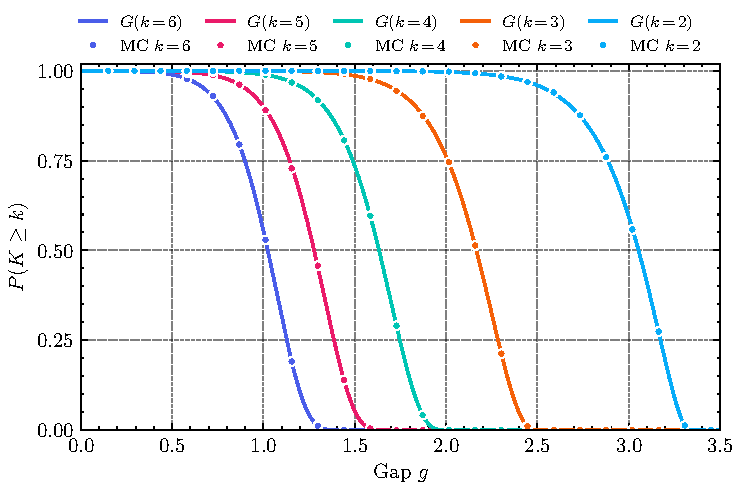
\includegraphics[width=0.78\linewidth]{figures/chain_probability.pdf}
    \caption{Validation of the two-boundary chain probability in~\eqref{eq:chain_prob}. Solid curves show the analytic expression $G(k;\lambda,L,g)$; markers show Monte Carlo estimates for the same anchored packing event.}
    \label{fig:chain_probability_validation}
\end{figure}


\end{document}
